\documentclass[a4paper,11pt]{report}
\usepackage{setspace}
\usepackage{fullpage}
\usepackage[square,sort&compress]{natbib}
%\usepackage[authoryear,sort&compress]{natbib}
\usepackage{tabu, longtable}
\usepackage{pdflscape}
\usepackage{bibentry}
\usepackage[table]{xcolor}
\usepackage{tablefootnote}
\usepackage{hyperref}
\usepackage{amsmath}
\usepackage{graphicx}
\usepackage{amssymb}\usepackage[T1, OT1]{fontenc}
\usepackage{hyperref}
\usepackage{subcaption}
\renewcommand{\dh}{\fontencoding{T1}\selectfont{\symbol{240}}}
\graphicspath{ {../pics/} }

%MACROS

%footnotes in tables
%\makesavenoteenv{tabular}

% shade rows in table
%\rowcolors{2}{gray!15}{white}

% alternate rowcolors for all tables
\let\oldtabular\tabular
\let\endoldtabular\endtabular
\renewenvironment{tabular}{\rowcolors{2}{white}{gray!15}\oldtabular}{\endoldtabular}

% alternate rowcolors for all long-tables
\let\oldlongtable\longtable
\let\endoldlongtable\endlongtable\renewenvironment{longtable}{\rowcolors{2}{white}{gray!15}\oldlongtable} {
\endoldlongtable}

% allow column widths in tables with alignment
\newcolumntype{L}[1]{>{\raggedright\let\newline\\\arraybackslash\hspace{0pt}}m{#1}}
\newcolumntype{C}[1]{>{\centering\let\newline\\\arraybackslash\hspace{0pt}}m{#1}}
\newcolumntype{R}[1]{>{\raggedleft\let\newline\\\arraybackslash\hspace{0pt}}m{#1}}

\onehalfspacing
% define the title
\author{Oliver S Burren}
\title{First Year Report - Draft}
\begin{document}
% generates the title
\maketitle

\begin{abstract}
 Genome wide association studies (GWAS) have uncovered hundreds of genetic regions that are responsible for human susceptibility to autoimmune disease.  Identification and functional characterisation of causal variation, a pre-requisite for therapeutic intervention, has proved difficult. This challenge stems both from the underlying complex genetic architectures that are refractory to the statistical resolution of causal variation, and the cryptic nature of the genes that such variation targets, due to tissue specific three dimensional (3D) chromatin organisation.  Recent empirical developments have enabled high resolution maps of 3D chromatin organisation to be elucidated using promoter capture Hi-C that might allow the physical linkage of causal variants with target  genes. The aim of my PhD is to develop statistical methods to integrate GWAS with these tissue specific PCHi-C maps and other genomic data in order to better understand the biology of autoimmue susceptibility.  
 
 Firstly, I developed \textit{blockshifter} a  competitive circularised permutation method for examing promter interacting regions (PIRs) for trait associated variant enrichment, that allows for correlation between variants and interactions. Applying \textit{blockshifter} to publicly available summary statistics for eight autoimmune and 23 non-autoimmune traits, and PCHi-C maps for 17 haematopoetic tissues I found enrichment for autoimmune variants in lymphoid tissues, which was strongest in activated CD$^+$ T cells. Next, I developed a Bayesian method, COGS, to generate PCHi-C supported gene scores to prioritise variants, genes and tissue contexts for functional validation.  I applied COGS to prioritise 2,604 genes across all 31 traits and tissues. COGS gene scores were more specific and sensitive when compared to similar methods using either proximal gene variants or topologically associated domain (TAD) boundaries. I found that genes prioritised by COGS were significantly enriched for genes differentially expressed between healthy and diseased immune subsets ($P = 0.002$ - ulcerative colitis). In contrast scores for TAD and proximal methods showed no enrichment. 
 
 Putatitve causal variation in a PIR in intron 1 of\textit{IL2RA}, prioritised by COGS in  in CD4$^+$ T cells across multiple autoimmune diseases was examined using allele specific expression (ASE). ASE was found in unstimulated CD4$^{+}$ T cells but was lost on stimulation, providing support for COGS prioritisation and the utility of PCHi-C maps for interpreting tissue context function. Future work will: a) explore approaches to the integration of other relevant genomic datasets, b) use simulated GWAS statistics to better characterise COGS scores. c) develop tissue specific gene set enrichment methods based on COGS scores.  
\end{abstract}
% insert the table of contents
\tableofcontents
\chapter{Introduction}
\section{Motivation}

A key property of the adaptive immune system is the ability to recognise pathogens from self-antigens.  Dysregulation of this process results in damage to healthy tissues and autoimmunity. Currently, over 80 diseases have been found to have an underlying autoimmune pathogenesis, with approximately half presenting as rare diseases~\citep{HayterCook2012}. The health burden of more common autoimmune diseases such as type 1 diabetes (T1D), rheumatoid arthritis (RA), inflammatory bowel disease (IBD) and multiple sclerosis (MS) is high with approximately 7 - 9$\%$ of the European population affected~\citep{CooperBynumSomers2009}. Although environment is a contributing factor in disease susceptibility, the genetic heritability, defined as the proportion of phenotypic variance attributable to genetic variability, is also important, ranging from 0.39 in primary billiary cirrhosis (PBC) to 0.9 in ankylosing spondilitis (AS)~\citep{Gutierrez-ArcelusRichRaychaudhuri2016}.  

Genome wide association studies (GWAS) have been instrumental in understanding the complex genetic architecture underlying autoimmune disease susceptibility with at least 324 distinct genetic loci robustly associated with one or more autoimmune diseases (\url{http://www.immunobase.org}, accessed $01/08/2016$). Focus is now drawn to elucidating the mechanisms by which underlying causal variation modulates phenotypic endpoints, a prerequisite for successful therapeutic development. Interestingly, the majority of associated variants fall outside of genes ~\citep{MauranoHumbertRynesEtAl2012} and the integrative analysis of chromatin marks with GWAS highlights a tissue specific specific regulatory role ~\citep{FarhMarsonZhuEtAl2015}.  Recent studies ~\citep{ClaussnitzerDankelKimEtAl2015,SmemoTenaKimEtAl2014,Davison2012-zk} have shown that such regulatory variants might, through chromatin conformation, regulate distal genes. However, further progress in this area has been hampered by incomplete knowledge of causal variants and their target genes and the specific tissue contexts in which they operate~\citep{Albert2015-jn}.

To date systematic methods for incorporating physical interactions between variants and their target genes have not been attempted. In this report I describe tools and analytical methods to integrate genetic and high resolution promoter capture Hi-C (PCHi-C). I focus method development on using GWAS summary statistics for input, as due to legitimate privacy concerns, access to raw genotype data is more restrictive, limiting the number of traits that can be analysed. These methods provide a data driven approache to prioritising putative causal variants underlying autoimmune disease susceptibility, and the relevant tissue contexts, genes and biological pathways within which they operate. I apply these methods to integrate 17 PHi-C maps for primary human cells with GWAS and fine mapping data across 31 traits. Based onthese results I extend this analysis to examine summary ImmunoChip dense mapping summary statistics for x autoimmune traits in the context of CD4${^+}$ T cell activation.

\section{Fine mapping}
One of the first steps of this project is to identify optimal methods for fine mapping, that balance data availibility, resolution and computational efficiency. Fine mapping is the process of refining association signals in a genomic region in order to characterise fine scale genetic architecture, a necessary step in order to identify putative causal variants. Progress in this area is challenging, due to the presence of linkage disequilibrium (LD), which in many cases means that the causal variation cannot be resolved statistically with current sample sizes. 

 One approach, under the simplifying assumption that a single causal variant explains the effect within a given genetic region, is to apply Wakefield's synthesis of approximate Bayes Factors (ABF)~\citep{Wakefield2009} to each variant within the region. These can be converted into posterior probabilities for a SNP to be causal using methods described in ~\citet{The_Wellcome_Trust_Case_Control_Consortium2012-ad}. A sizeable benefit of this approach is that it circumvents privacy issues, as the input is limited to GWAS summary statistics rather than access to full genotyping data.

Wakefield defines the ABF as

\begin{equation}
	ABF =  \sqrt{1 - r} \times \exp{\left[\frac{Z^{2}}{2} \times r\right]}
\end{equation}

If a given set of summary statistics include $\hat{\beta}$, an  estimate of the $\log(\text{Odds Ratio})$ and $\sqrt{V}$, the standard error of the Odds Ratio for a variant, then we can compute a $Z$ score such that $Z= \frac{\hat{\beta}}{\sqrt{V}}$. Alternatively, if only univariate $p$-values are supplied a $Z$ score can be estimated using an inverse normal cumulative distribution function . If $r$, a shrinkage factor, is defined as the  the ratio of the prior variance on $\hat{\beta}$ to the total variance, then, $r = \frac{W}{V + W}$. $V$ is approximated using the variant minor allele frequency (MAF) and study sample size such that $V=\frac{1}{2Nf(1-f)}$ for quantitiative traits, where $N$ is number of samples and $f$ is the MAF. In the case/control setting $V=\frac{1}{2Nf(1-f)s(1-s)}$ where $s$ is the proportion of cases . The value of $\sqrt{W}$, the standard deviation of a normal prior, depends on study design considerations. In this report we use values of 0.15 and 0.2 for  case/control  and quantitative trait settings  respectively, as discussed by \citet{GiambartolomeiVukcevicSchadtEtAl2014}.

Given the ABF for all SNPs in a given genetic block we can estimate the posterior probability that a SNP $i$  is causal using the following. 
% add equation here with an explanation
\begin{equation}
\label{form:bf_derivation}
\begin{split}
	PP_{i}& = P(\text{SNP}_{i}\text{ causal} | D)\\
	& = \frac{P(D | \text{SNP}_{i} \text{ causal})\pi_{i}}{\sum_{j}P(D | \text{SNP}_{j}\text{causal})\pi_{j} + P(D | H_{0})\pi_0}\\
	& = \frac{
				\frac{
					P(D | \text{SNP}_{i}\text{ causal})
				}
				{
					P(D|H_{0})
				}\pi_{i}
		}
		{
				\sum_{j=1}^n\frac{
					P(D | \text{SNP}_{j}\text{ causal})
				}
				{
					P(D|H_{0})
				}\pi_{j}  + \pi_0
		}	\\
	& = \frac{
		\text{BF}_{i}\pi_{i}
	}
	{
	\sum_{j=1}^n\text{BF}_{j}\pi_{j} + \pi_{0}
	} \\	
	\\
	& \approx \frac{
		\text{BF}_{i}\pi_{i}
	}
	{
	\sum_{j=1}^n\text{BF}_{j}\pi_{j} + 1
	} \\
\end{split}
\end{equation}
Note that as $\pi_{0} = 1-\sum_{j}\pi_{j} \approx 1$. 

$\pi_{i}$ is our prior probability for any SNP selected at random to be causal for a trait. Current sample sizes are underpowered and therefore have limited resolution. This has driven the the development of integrative techniques that couple fine mapping methods with functional information to further prioritise causal variants. Examples include \textit{fgwas}~\citep{Pickrell2014-xs}, PAINTOR~\citep{KichaevYangLindstromEtAl2014}, RiVIERA~\citep{LiKellis2016}   and the integration of eQTL data sets using Mendelian randomisation~\citep{ZhuZhangHuEtAl2016}. As an example ~\citet{Pickrell2014-xs} developed a Bayesian hierarchical frameworks implemented in \textit{fgwas} that estimates variable priors for each SNP based on other sources of annotation. For a given SNP the prior probability for association, $\pi_{ik}$, varies depending on the enrichment of annotations, $\lambda_{l}$. 

\begin{equation}
	\pi_{ik} = \frac{e^{x_{i}}}{\sum_{j \in S_k}e^{x_{j}}}
	\label{eqn:fgwas_var_prior}
\end{equation}

$x_i$ is the sum of the effect of all the annotations that the $i^{th}$ SNP overlaps as shown below.  Here $\lambda{i}$ is the effect of annotation $l$ and $I_{il}$ is and indicator function as to whether SNP $i$ overlaps annotation $l$.  

\begin{equation}
	x_{i} = \sum_{l=1}^{L_{2}} \lambda_{l}I_{il}
	\label{eqn:fgwas_lambda}
\end{equation}

$\lambda_{l}$ is itself of interest as it indicates whether a given annotation is enriched for association with a trait of interest. When combined with equation \ref{form:bf_derivation} $\pi_{ik}$ allows the incorporation of functional information with genetic data allowing a modest increase in resolution and a resultant decrease in the number of causal SNPs to be considered~\citep{Pickrell2014-xs}. Whilst promising \textit{fgwas} requires careful cross-validation to prevent overfitting whereby the derived model is biased for the training set but performs poorly on a test set of data, and all such methods are limited by the annotations available.

If raw genotyping data for a study is available then stepwise regression could be used, however whilst this approach is attractive computationally, doubts exist over it's validity~\citep{miller-1984}. Effectively having selected a single variant that best explains the variance of a trait, stepwise regression then looks for other variants that explain additional trait variance conditional on this `top' variant. This is not equivalent to explaining which variants jointly explain the variance of a trait. However, approaches that search the model space exhaustively are only computationally feasible for simple models incorporating a limited number of variants. An alternative approach is to use Monte Carlo methods to sample the model space allowing the consideration of multiple causal variants within a genetic region. One example is GUESSFM that uses a Bayesian evolutionary stochastic search algorithm to effectively sample the model space, and has been shown to have consistently better performance when variants are highly correlated~\cite{WallaceCutlerPontikosEtAl2015}. 

\section{Variant set enrichment}
The next part of my project investigates whether the putative causal SNPs identified can be used to better understand the biology of autoimmune disease.  If these variants  are enriched for a particular annotation or gene set then this can provide global information on mechanisms, relevant tissue contexts and biological pathways. However this is complicated by both correlation between variants (due to linkage disequillibrium) and annotations. 

\begin{equation}
	\text{Var}(A + B) = \text{Var}(A) + \text{Var}(B) + 2\text{Cov}(A,B)
\end{equation}

If $A$ and $B$ are non independent variables then the covariance term $2\text{Cov}(A,B)$ can be almost as large as $\text{Var}(A) + \text{Var}(B)$. This causes the observed variance to be inflated compared to the theoretical variance if independence is assumed. Unfortunately most classical statistical tests based on linear sums of variables assume independence and thus the inflated variance of the computed test statistic increases type 1 error, that is the erroneous rejection of the null hypothesis. Permutation based methods, that can use GWAS summary statistcs are desirable as they can help to overcome this inflation by estimating the variance emprically. There are two broad permution methods, firstly, using a suitable reference genotype set to compute covariance matrices allows the estimation of SNP variance under the null hypothesis using the multivariate normal~\cite{LiuMcRaeNyholtEtAl2010,Burren2014-vh}. These approaches are computationally expensive and scale exponentially with SNP density, thus an LD pruning strategy is employed which limits resolution and therefore is only applicable to larger genomic annotations such as genes. The second approach is to permute the annotations over the SNPs whilst maintaining the spatial correlation structure of the target annotation to estimate the variance under the null. The latter approach is attractive as it favours high resolution annotations and is computationally more tractable. GOSHIFTER is a recent implementation using a circular permutation strategy ~\citep{Trynka2015-wz} that demonstrates this approach finding enrichment for H3K4me3 marks in CD$+$ memory T cells. 

As previously mentioned integrative approaches such as \textit{fgwas} combine variant set enrichment with fine mapping strategies to simultaneously prioritise annotations and variants. This approach additionally benefits from jointly assessing multiple annotations, thus if there is additional correlation between different annotation types this can be adjusted for.  It should be noted that all methods are dependent on the quality and coverage of input annotations. A recent study fine mapping IBD causal variants found that 21 variants with extremely high probability ($>$ 95$\%$) to be causal did not overlap any functional annotations, drawing attention to the inadequacies of current genomic functional annotation~\citep{Huang2015-ug}.

%We used a prior ($\pi_{i}$) of $10^{-4}$ which means that we expect 1 in 10,000 SNPs to be causal for a trait
\section{High resolution promoter capture Hi-C}
The most novel aspect of this project is using a data driven approach to link putative causal variation to the target genes in relevent tissues. Techniques such as Hi-C~\citep{Lieberman-AidenvanBerkumWilliamsEtAl2009} and  Chromatin Interaction Analysis by Paired-End Tag Sequencing (ChIA-PET)~\citep{FullwoodLiuPanEtAl2009} have been developed to map the genome-wide chromatin interactions in specific cell types~\citep{RaoHuntleyDurandEtAl2014}. Hi-C involves cross-linking genomic DNA with formaldehyde resuting in covalent links between spatially adjacent chromatin segments. This chromatin is then digested with a restricition enzyme and sticky ends are filled in with biotin labelled nucleotides. Ligation is then performed under dilute conditions which favours intramolecular ligation events. The DNA is then purified and then sonically sheared and fragments are then enriched for biotinylated junctions, which then undergo paired end sequencing~\citep{vanBerkumLieberman-AidenWilliamsEtAl2010}. ChiA-PET again involves using formaldehyde to covalently link spatially adjacent chromatin. After sonification an immunoprecipitation step is used select a protein of interest (e.g. transcription factor) and the chromain to which it is bound. Next biotin conjugated linker sequences are ligated to the free ends of the immunoprecipitated DNA. A further proximity based ligation takes place with enrichment of biotinylated linkers. Barcodes within the linker sequences are used to resolve chimeric intra and inter complex interactions. 

Whilst both are genome-wide methods for interrogating chromatin looping, CHiA-PET targets a specific protein and therefore compared to Hi-C is unable to give an unbiased overview of all chromatin interactions within a given tissue context. However, Hi-C resolution is limited by two main factors. Firstly the protocol involves a restriction enzyme digest, usually \textit{Hind}III, and interactions are called based on the resultant fragments generated, in practice if \textit{Hind}III is is used this limits resolution to approximately 4Kb. Secondly,  the complexity of the sequence libraries generated means that to increase the effective resolution of conventional Hi-C by a factor $n$ requires $n^{2}$ sequencing reads which is prohibitive for general implementation~\citep{JaegerMiglioriniHenrionEtAl2015}. Promoter capture Hi-C (PCHi-C) incorporates a sequence capture extension to classical Hi-C to enrich for chromatin interactions with protein coding gene promoters~\citep{Mifsud2015-fm}. Such PCHi-C allows for increasing resolution in an approximately linear fashion with increased sequence depth allowing for an economically viable approach for identifying promoter interactions. 

%\section{Aims}


%My main aim is to understand whether PCHi-C can provide a better understanding of how causal variation modulates autoimmune disease. For convenience this can be subdivided into answering three specific questions:

%\begin{enumerate}
%	\item Can PCHi-C help us to identify causal variation ?
%	\item What information can PCHi-C provide about genes and cellular contexts modulated by causal variants ?
%	\item Can these genes and cellular contexts identify novel pathways that inform the biology of autoimmunity ? 
%\end{enumerate}

%In this report I describe the development of a methodological framework that can be used to integrate tissue specific PCHi-C interaction maps with both targeted and genome wide genetic studies. Using a set of interaction maps for 17 haematopoietic primary Human cell types and focusing on autoimmunity I use this framework to define lists of prioritised variants, genes and cellular contexts. I show how these can be further refined by using  deep genomic phenotyping of  CD4$^{+}$ T cells  in activated and non-activated states. Finally I discuss followup experiments in \textit{IL2RA} that demonstrate context specific allelic imbalance, that provides validation of this framework.

\chapter{Materials and Methods}

\section{Promoter capture interaction maps of 17 haematopoetic primary human cells}
I obtained maps of 17 primary human cells of the haematopoetic lineage that were generated collaboratively with members of the Fraser, Spivakov, Ouwehand and Diabetes and Inflammation Laboratories. Each cell type was assessed over on average 3 technical replicates (Table \ref{tab:pints}). The bespoke capture platform employed encompassed a total of 22,076 \textit{Hind}III fragments containing 31,253 annotated promoters for 18,202 protein-coding and 10,929 non-protein coding genes (Ensembl v75). Significantly interacting regions were called using the CHiCAGO pipeline~\citep{CairnsFreire-PritchettWingettEtAl2016}. Interactions with a CHiCAGO score threshold of $\geqslant$ 5 were used in all downstream analysis. These maps consist of a bait \textit{Hind}III fragment and a list of interacting \textit{HindIII} fragments or promoter interacting regions (PIR) within a particular cellular context.

\section{Collection and quality control of GWAS summary statistics from 31 genome wide association studies}
I downloaded GWAS summary statistics, covering 8 autoimmune and 23 other traits, from online resources, as detailed in Table\ref{tab:gwasm}. Genotyping error can create false associations,  therefore I filtered all association statistics to include only robust associations by removing those SNPs which were genome-wide significant ($p < 5 \times 10^{-8}$) but for which no variants, within 500Kb, in LD ($r^{2} > 0.6$) with the lead SNP had $p < 1 \times 10^{-5}$. Finally I removed any SNP that was genome-wide significant but was not found in the 1000 Genomes PhaseIII EUR genotype set. 
%This code is found in gwas_integration/R/QC.R
\section{Poor Man's Imputation (PMI) - Imputation of GWAS p-values to the 1000 Genome reference panel in the absence of effect size and direction}
There was a high degree of variation in the coverage of GWAS summary statistics obtained, some studies contained information on approximately $5 \times 10^5$ variants where as others were imputed to 1000 genome reference genotype set and contained in excess of $7 \times 10^6$ variants. Imputation can be used to compute approximate association statistics for missing variants however it requires access to underlying genotype data which in this case was unavailable for most traits. Methods exist for imputing summary statistics in the absence of genotyping data such as \textit{GCTA}~\citep{YangLeeGoddardEtAl2011} and \textit{IMPG}~\citep{Pasaniuc2014-im}, however these rely on access to odds ratio or $\beta$ coefficients and their standard errors to estimate direction of effect which are not always available. I therefore designed an alternative `best guess' method, poor man's imputation (PMI), which requires evaluation but allows the processing of a wide range of traits for which variant coverage is heterogeneous and only univariate $p$ values are available.

The pipeline I developed, approximates the $p$-value for missing SNP summary statistics for a given study using a suitable reference genotype set. Firstly the genome is split into regions based on a recombination frequency of 0.1cM using HapMap recombination rate data. For each region we retrieve from the reference genotype set (1000 genomes EUR cohort) all SNPs that have MAF $ > 1\%$ and use these to compute pairwise LD. The pipeline pairs each SNP with missing $p$-values to the SNP with maximum pairwise $r^2$, ${r^2}_{max}$, if that ${r^2}_{max} > 0.6$, and impute the missing $p$-value as that at the paired SNP. SNPs with missing data or without a pair above threshold are discarded as are SNPs that are included in the study but do not map to the reference genotype set.

\section{Causal variant posterior probabilities for 31 traits using GWAS summary statistics}
To fine map candidate causal variants I used Wakefield's synthesis of approximate Bayes factors (ABF)~\citep{Wakefield2009} and using the method described in \citet{The_Wellcome_Trust_Case_Control_Consortium2012-ad} computed posterior probabilities for each SNP within 0.1 cM regions, using R code adapted from the \textit{coloc} package~\citep{GiambartolomeiVukcevicSchadtEtAl2014}.  

I set the value of prior of the $i^\text{th}$ variant being causal ($\pi_{i}$) to that from \citet{GiambartolomeiVukcevicSchadtEtAl2014}, $10^{-4}$, which means that we expect 1 in 10,000 SNPs to be causal for a trait. This framework assumes a model where either no SNPs are causal within a region or that exactly one SNP is causal. We masked the MHC region (GRCh37:chr6:25-35Mb) from all downstream analysis due to its extended LD and known strong and complex association with autoimmune diseases

\section{Comparison of posterior probabilities between PMI and classical imputation}
Before using PMI posterior probabilities in further analyses it was neccessary to assess whether they approximated posterior probabilities derived from classiscal imputation. Firstly I selected all SNPs mapping to Chromosome 1 as a representative sample. To create a simulated non-imputed data set I pruned these results to contain only SNPs for which p-values were reported in ~\citet{Stahl2010-wz}. I next ran PMI on this pruned data set and using \textit{bedtools}~\citep{Quinlan2014}, merged these with actual the imputed p-values from~\citet{Okada2014-um}. I confined my comparison to those SNPs imputed by PMI, a total of 235,412 SNPs

\
%\section{Variant posterior probabilities of inclusion using full genotyping data}

%For four diseases (autoimmune thyroid disease, celiac disease , rheumatoid arthritis and type 1 diabetes) we had access to full genotyping data from ImmunoChip. Chris Wallace carried out formal imputation to 1000 genomes project EUR using IMPUTE2 and fine mapped causal variants in each of the 179 regions where p$<$0.0001 was observed using a stochastic search method that allows for multiple causal variants within a region~\citep{WallaceCutlerPontikosEtAl2015}. 

\section{blockshifter - A competitive test for associated variant enrichment in PCHiC interaction maps}
In order to examine the enrichment of GWAS signals in promoter interacting regions (PIRs) I developed a method based on ideas implemented in \textit{GOSHIFTER}~\citep{Trynka2015-wz} to examine the enrichment of GWAS signals in the promoter interacting regions (PIR) in order to overcome linkage disequilibrium (LD) and interaction fragment correlation. \textit{blockshifter} implements a competitive test of enrichment between a test set of PIRs compared to a control set. Firstly the coordinates of the PIRs in the union of test and control sets are retrieved, and PIRs with no overlapping GWAS signal  are discarded. As the test is competitive between PIRs in test and control sets, those overlapping both are not informative and therefore are excluded from further analysis. For the remaining PIRs we store the number and sum of overlapping GWAS posterior probabilities and these are used to compute $\delta$, the difference in the means of posterior probabilities between the test and control set . Due to correlation between GWAS signals and between PIRs the variance of $\delta$ is inflated, we estimate it empirically using permutation.  Runs of one or more PIRs (separated by at most one \textit{Hind}III fragment) are combined into ‘blocks’, that are labeled unmixed (either test or control PIRs) or mixed (block contains both test and control PIRs).  Unmixed blocks are permuted in a standard fashion by reassigning either test or control labels randomly across blocks taking into account the number of blocks in the observed sets. Mixed blocks are permuted by effectively circularising each block and rotating the labels (figure \ref{fig:blockshifter}). I store the mean posterior probabilities across each possible permuted block. The number of choices at each block is small, but there are many blocks. I then randomly sample from each these precomputed block permutations $n$ times so that the proportion of underlying PIRs labels is the same as the observed set and use this to compute the set of $\delta_{null}$. I use $\delta_{null}$ to compute an empirical $Z$-score:
\begin{equation}
Z = \frac{\delta - \bar{\delta_{null}}}{\sqrt{V*}}
\end{equation}
Where $V^{*}$ is an empirical estimate of the variance of $\delta_{null}$. 

\begin{figure}[h]

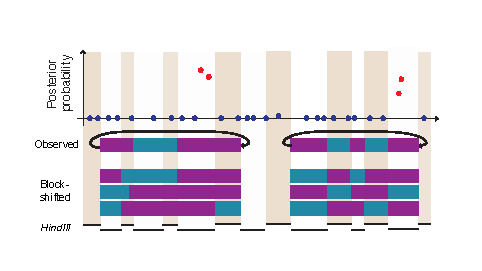
\includegraphics[width=\textwidth]{blockshifter.pdf}
\caption{Illustration of circularised permutation method for mixed `superblocks'. Test(Purple) and Control(Turquoise) tissue PIRs are rotated to generate permutations, \textit{Hind}III fragments with no PIRs (grey) are fixed.}
\label{fig:blockshifter}
\centering
\end{figure}

\section{COGS - An algorithm for PCHiC assisted prioritisation of genes and tissues contexts}
Whilst the blockshifter method provides information about relevant tissue contexts, the primary goal of this project is to use the PCHi-C information to link causal variation to target gene(s). To do this
I developed an algorithm to compute tissue specific gene scores for each GWAS trait, taking into account linkage disequilibrium, interactions and functional SNP annotation (figure \ref{fig:cogs}). For each gene annotation, for which we have at least one significant interaction and for every nearby recombination block, the algorithm computes a block gene score that is composed of three components.

\begin{figure}[h]
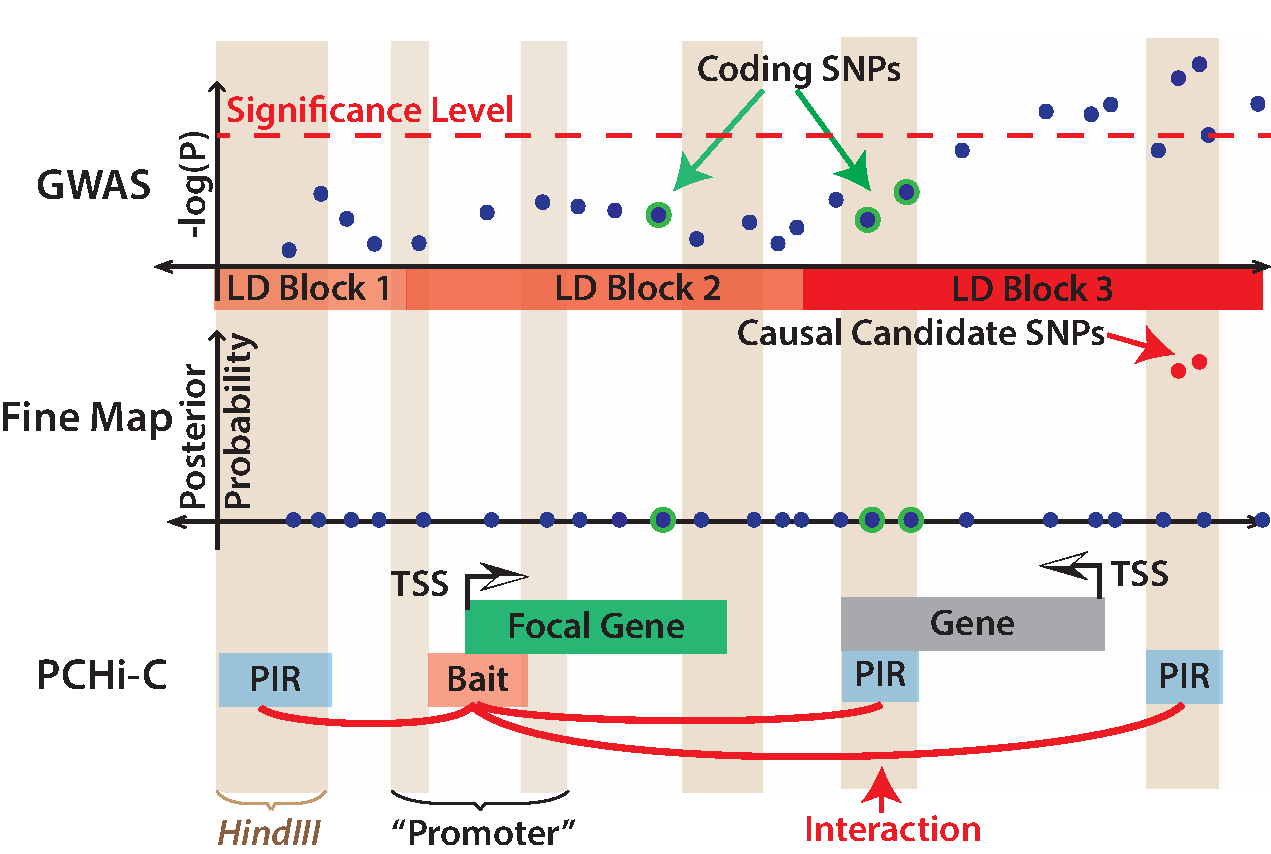
\includegraphics[width=\textwidth]{cogs3.pdf}
\caption{A schematic illustration of the COGS method. GWAS summary stastics are imputed by PMI and converted to posterior probabilities (PPI) across three linkage disequillibrium (LD) blocks. These are then intersected with PCHi-C maps, promoter interacting regions and their linkages to bait \textit{Hind}III fragments allow the assignment of posterior probabilities to a focal gene (green). Due to limitiations in the ability to call very short range interactions we create `Promoter' regions that consist of bait and adjoining \textit{Hind}III fragments. We account for protein coding SNPs by considering those in the focial gene (green) and masking others. Assuming independence between LD blocks we sum the information across categories to compute an overall gene score. In the above example naive analysis might prioritse a non focal gene (grey), however PCHi-C interactions provide additional information supporting the focal gene.}
\label{fig:cogs}
\centering
\end{figure}

\begin{enumerate}
\item The contribution due to coding SNPs in the annotated coding gene as computed by VEP.
\item The contribution due to promoter SNPs, which I define as SNPs that overlap the bait and it's pair of flanking \textit{Hind}III fragments and not any coding SNPs.
\item The contribution due to SNPs that overlap interacting other ends for a tissue or set of tissues that do not overlap coding SNPs. 
\end{enumerate}

For a given target gene and recombination block the algorithm derives a block gene score that is the sum of the posterior probabilities of SNPs overlapping each component, which is the probability that there exists a causal variant for this gene in this block, under the assumption that there is at most one causal variant in any block. Assuming independence we can combine blocks to get an overall gene score such that:

\begin{equation}
  Gene\ score = 1- \prod_j  \left(1-\left(\sum_{i \in R_j} 1-PP_i \right) \right)
  \label{eqn:cogs_score}
\end{equation}

Here $PP_i$ is the posterior probability for the $i^{th}$ variant to be causal, $i \in R_j$ is the set of relevant SNPs $i$ in the $j^{th}$ region. Whilst components 1 and 2 are fixed for a given gene and trait the contribution of variants overlapping PIRs varies depending on the tissue context being examined. I developed a hierarchical heuristic method to ascertain for each target gene which was the mostly likely component and cell state. Firstly for each gene I compute the gene score due to genic effects (components 1 $+$ 2) and interactions (component 3) using all available tissue interactions for that gene. I use the ratio of gene effects score to interactions score in a similar manner to a Bayes factor to decide whether one is more likely. If gene effect is more likely (ratio $>$3) I iterate and compare if the gene score due to coding variants (component 1) is more likely than for promoter variants (component 2). Similarly if an interaction is more likely I compare interaction gene scores for one set of tissue(s) to another. If at any stage no branch is substantially preferred over its competitor (ratio of gene scores $<$ 3) I return the previous set as most likely, otherwise I continue until a single cell state/set is chosen. In this way I can prioritise genes based on the overall score and label a likely mechanism for candidate causal variants (\ref{fig:AHR_dend}).

For the four traits where a stochastic search method was employed I adapted COGS to work with multiple models by aggregating the posterior probabilities for each model with a variant overlapping the PIRs, promoters or coding variants to compute marginal posterior probabilities of inclusion.

\section{Comparison of COGS scores to non PCHi-C methods}
To assess the utility of COGS scores and whether PCHi-C datasets were adding information, I generated comparitve scores using two other methods orthoganol to PCHi-C. The intent behind this analysis is to assess the utility of interaction data and therefore as input to all methods I supplied PMI datasets from which I had masked coding variation and variation mapping the MHC region on chromosome six. Firstly, I had access to topological associated domain (TAD) boundary information, supplied by Csilla Varnai, Michiel Thieke and Mikhail Spivakov for six cell types (Table \ref{tab:hic_coverage}). I integrated these with the 0.1cM recombination block data used to compute posterior probabilities. For each intersection between LD block and TAD  I summed posterior probabilities, and computed a summary posterior probability for each TAD and tissue combination using equation \ref{eqn:cogs_score}. I assigned these scores to protein coding genes based on overlap between baited gene fragments. For this analysis I combined across tissues by taking the maximum TAD score for a gene.

Secondly, I created gene scores based on proximity of associated variants to gene promoters. I took all \textit{Hind}III fragments within $\pm$ 0.5 Mb of a genes baited gene \textit{Hind}III and assigned to LD fragments in a similar fashion to TAD score computation detailed above. Finally I computed a comparison COGS score using only PCHi-C maps for  tissues for which TAD boundary information were available (Table \ref{tab:hic_coverage}).

\begin{table}[ht]
\centering
\begin{tabular}{cc}
  \hline
 Tissue & TAD Coverage (Gb) \\ 
  \hline
Erythroblasts & 1.53 \\ 
  Macrophages & 1.68 \\ 
  Megakaryocytes & 1.59 \\ 
  Monocytes & 1.48 \\ 
  Naive B cells & 1.51 \\ 
  Naive CD4$^+$ T cells & 1.40 \\ 
  Naive CD8$^+$ T cells & 1.51 \\ 
  Neutrophils & 1.27 \\ 
   \hline
\end{tabular}
\label{tab:hic_coverage}
\caption{Topologically associated domain coverage across eight cell types elucidated from classical Hi-C analysis}
\end{table}

\section{Enrichment of COGS in disease specific differentially expressed genes}
As a naive method to assess the biological relevance of the genes prioritised by COGS and to allow quantitative comparison between the TAD, Proximity and COGS methods, I examined  differentially expressed genes from \citet{PetersLyonsLeeEtAl2016} for enrichment of genes prioritised on the basis of the different methods. To do this I used differential expression analysis supplied by Chris Wallace. The dataset consists of PEER normalised microarray expression values across 49 patients with Crohn's disease, 42 with ulcerative colitis and 43 healthy controls, across sorted  CD4$^+$ T cells, CD8$+$ T cells, B cells, monocytes, and neutrophils. Differential expression was computed with a null hypothesis that expression for a given gene was the same across all three groups within a tissue. As COGS and TAD scores are derived by combining over cell types we selected the tissue with the maximum significant differential expression values across tissue for a given gene. As the differential expression analysis concerned ulcerative colitis and Crohn's disease we used as input GWAS statistcs from \citet{Anderson2011-ch} and \citet{Franke2010-mj} with coding and MHC variants removed.

\section{Causal variant posterior probabilities for using ImmunoChip summary statistics}
Dense genotyping platforms target specific genomic regions to provide higher resolution genetic maps. I wanted to see, in the context of activated and non activated CD4$^{+}$ T cells, what extra information could be gained by integration of PCHi-C maps with genetic data from such targeted studies.  Focusing on Autoimmune traits,  I downloaded  ImmunoChip summary statistics for six traits from \url{http://www.immunobase.org} carrying out QC as previously described. The ImmunoChip is a targeted genotyping platform for dense coverage of approximately 180 regions with robust demonstration of association with one or more autoimmune traits~\citep{CortesBrown2011}. Summary statistics for ulcerative colitis, Crohn's disease and psoriasis were supplied privately by study authors. I fine mapped these traits using the PMI method previously described, but replacing 0.1cM regions with the 179 regions (median size 227Kb with an inter quartiile range of between 126Kb and 392Kb) that were densely genotyped on the ImmunoChip~\citep{Onengut-Gumuscu2015-lb}. 

\section{Comparison of PMI with genotype method allowing for multiple causal variants in a region}

To evaluate the effect on COGS scores of the PMI  assumption of a single causal variant I used a set of marginal posterior probabilities obtained by Chris Wallace using a stochastic search method that allows for multiple causal variants within a region~\citep{WallaceCutlerPontikosEtAl2015}. I compared  four diseases(autoimmune thyroid disease, celiac disease , rheumatoid arthritis and type 1 diabetes)   for which we had access for full genotyping data from ImmunoChip and summary statistics. I incorporated these into further analysis on the assumption that full gentotyping data and imputation would provide more accurate posterior probabilities at the targetted regions.



%Whilst components 1 and 2 are fixed for a given gene and trait the contribution of SNPs overlapping PIRs varies depending on the tissue context being examined. We developed a hierarchical heuristic method based on the Haematopoietic tree to ascertain for each target gene which was the mostly likely component and tissue context. Firstly for each gene we compute the gene score due to gene effects (components 1 + 2) and interactions (component 3) using all available tissue interactions for that gene. We use the ratio of gene effects score to interactions score in a similar manner to a Bayes factor to decide whether one is more likely. If gene effect is more likely we iterate and compare if the gene score due to coding SNPs (component 1) is more likely than for promoter SNPs (component 2). Similarly if an interaction is more likely we begin descending the Hematopoietic tree and compare interaction gene scores for sets of tissues (e.g Myeloid vs Lymphoid). If at any stage the algorithm is unable to choose it stops and return the previous set as most likely, otherwise it continues until a single tissue/set is chosen. In this way we can prioritize genes based on the overall score and label as to a likely mechanism for candidate causal variants.

\section{Reactome Pathway Analysis}
Using modified R code developed by Mikhail Spivakov, for each trait I selected all protein coding genes having an overall gene score above 0.5. I converted Ensembl gene identifiers to Entrez gene indentifiers using bioMaRT~\citep{DurinckSpellmanBirneyEtAl2009} and used ReactomePA~\citep{YuHe2016} to compute the enrichment of genes within the Reactome pathways using an FDR cutoff of 0.05, using ClusterProfiler~\citep{YuWangHanEtAl2012} to plot a bubble plot of significant results.  


%\section{Tissue specific HALLMARK gene set enrichment analysis}
%Using modified R code developed by Chris Wallace  I used Wilcoxon rank sum tests to compare the distribution of gene prioritisation scores for genes in each MSigDB HALLMARK~\citep{LiberzonBirgerThorvaldsdottirEtAl2015} set to its complement, within the set of genes that both had membership of at least one HALLMARK set and had a gene score.  I used the $p$ value from this test, together with the difference in mean gene prioritisation scores, to generate a signed $Z$ score, $Z_{ig}$ for trait $i$ and gene set $g$.  To test for relative enrichment in autoimmune diseases versus non-autoimmune traits, we used $t$ tests to compare the distributions of $Z_{ig}$ for $i$ indexing autoimmune diseases to the $Z_{jg}$ for $j$ indexing non-autoimmune traits.

%\section{IL2RA allelic imbalance}

%Move to the discussion
%Targetted sequencing of \textit{IL2RA} in CD4$^{+}$ T cells was carried out, by Daniel Rainbow, across four donors that were heterozygous at eight group A SNPs and homozygous for group C and F SNPs (Figure\ref{fig:il2ra_ase}). This was carried out at 0, 2 and 4 hours after stimulation. Data processing was carried out using the Methpup package ~\citep{RainbowYangBurrenEtAl2015} (https://github.com/ollyburren/Methpup) to extract counts of each allele at rs61839660. Chris Wallace carried out the statistical analysis of the results. Briefly, the fraction of A2/(A1+A2) was compared across replicates in each cDNA sample to gDNA within individuals using Wilcoxon rank sum tests.  Where there was a bias in the same direction in each individual, combined p values were generated across individuals using Fisher’s product of p values method.   


\chapter{Results}

\section{Comparison of PMI with genotype level imputation}

To validate performance of the PMI technique, I compared the results as imputed by PMI to those as reported by  ~\citep{Okada2014-um}. There was good agreement between PMI imputed p-values and those derived from classical imputation as reported in~\citet{Okada2014-um} ($\rho=0.9418103$, figure \ref{fig:pmi_comparison}). % need to add something about why they are sometimes different and how this relates to MAF ?

\begin{figure}[h]
\centering
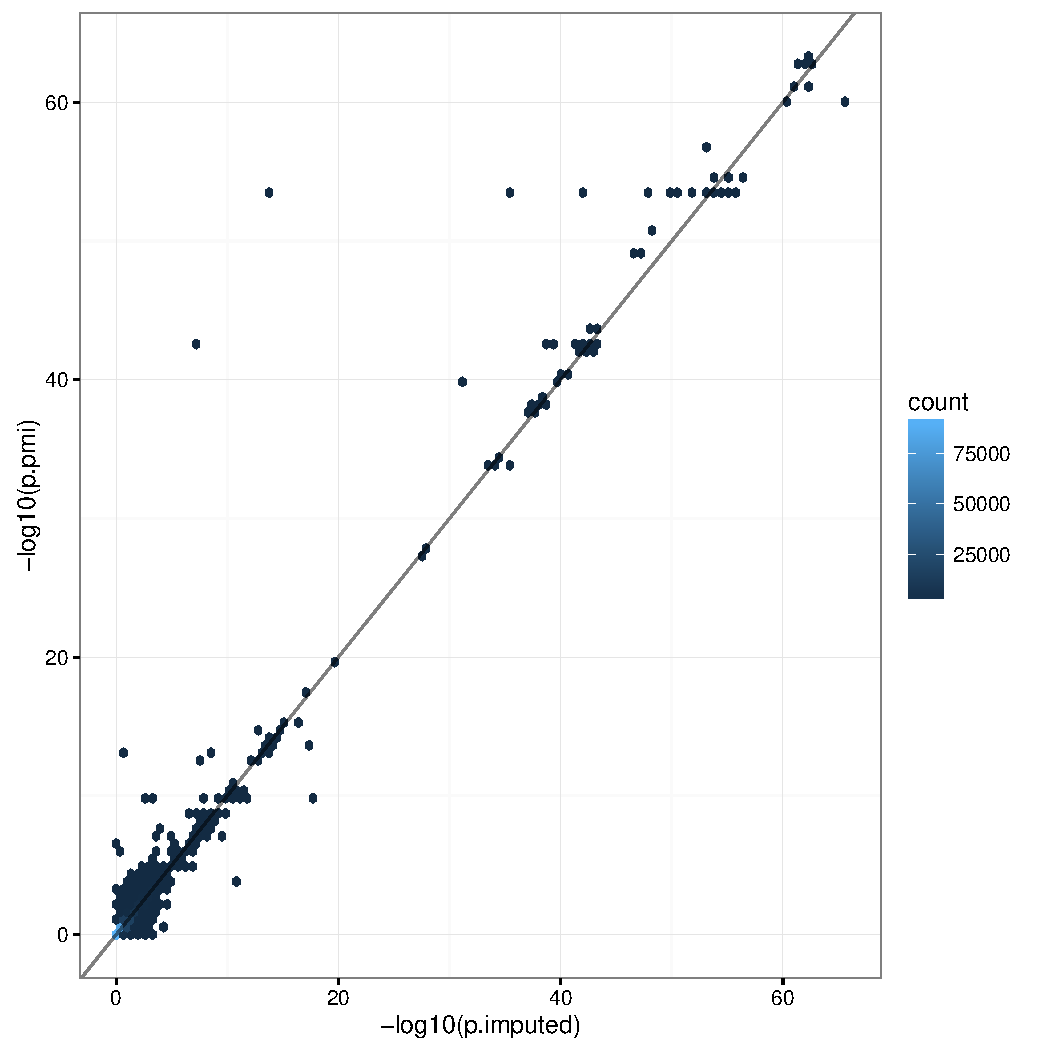
\includegraphics[width=0.8\textwidth]{pmi_vs_imp.pdf}
\caption{Comparison of $P$-values imputed by PMI versus those reported in ~\citep{Okada2014-um} for chromosome. Axis are $-\log_{10}$ transformed $P$-values}
\label{fig:pmi_comparison}
\end{figure}

%\subsection{Generation of Promoter Capture Hi-C interaction maps across 17 primary human cell types}
%Promoter Capture Hi-C interaction maps for 17 primary human cell types were generated as part of a collaboration between the Diabetes and Inflammation Laboratory(DIL), Fraser and Spivakov Groups and the BLUEPRINT consortium. Significant interactions were called using CHiCAGO~\citep{CairnsFreire-PritchettWingettEtAl2016} (Table\ref{tab:pints}) and these were then reannotated to EnsEMBL 75 using \textit{bedtools}~\citep{Quinlan2014}. To enable visual inspection of these results alongside GWAS summary statistics we developed the CHiCP~\citep{SchofieldCarverAchuthanEtAl2016} (https://www.chicp.org) webserver. 

%\subsection{Fine mapping of  GWAS summary statistics across 31 traits}
%We created a compendium of GWAS summary statistics from a vareity of sources for 31 traits (Table\ref{tab:gwasm}). In order to maximise resolution and coverage we imputed to 1000 Genome Phase III reference genotype set ~\citep{1000_Genomes_Project_Consortium2015-wc}. Compare PMI to Imputed. 
%Many studies were missing direction of effect statistics precluding the use of existing summary statistics imputation methods such as  \textit{ImpG}~\citep{Pasaniuc2014-im}. We therefore developed an LD based approach, which we named Poor Man's Imputation (PMI).We used Wakefield's~\citep{Wakefield2009} synthesis of approximate Bayes factors to compute posterior probabilities for a single variant being causal, within 0.1cM recombination blocks. We masked the MHC region (GRCh37:chr6:25-35Mb) from all downstream analysis due to its extended LD and known strong and complex association with autoimmune diseases.

\section{Tissue specific enrichment of associated variants with PIRs across 31 traits}
Enrichment of GWAS signals in tissue specific enhancers has been previously described~\citep{MauranoHumbertRynesEtAl2012} and as we expect PIRs to be enriched for regulatory regions. As such demonstration of robust enrichment, within tissue specific PIRs, is a pre-requisite for further analysis that attempts to link causal variation to target genes in relevent tissue contexts.  Using \textit{blockshifter} with the PMI imputed summary statistics from the 31 GWAS assembled (Table\ref{tab:gwasm}), I found that variants associated with autoimmune disease are enriched in PIRs in lymphoid compared to myeloid tissues (figure \ref{fig:bs_1}). In contrast, SNPs associated with erythroid traits, including mean haemoglobin concentration (MCH), mean corpuscular volume (MCV) and red blood cell count (RBC) showed a selective enrichment in erythroblasts and megakaryocytes compared to PIRs in monocytes, macrophages and neutrophils (figure \ref{fig:bs_1}). I next examined whether I could further resolve tissue differences using \textit{blockshifter}. I found that autoimmune traits were enriched in activated and non-activated CD4$^{+}$ T cells when compared to megakaryocytes and erythroblasts. This enrichment for autoimmune disease traits was stronger in activated  compared to non activated CD4$^{+}$ T cells (figure \ref{fig:bs_2}).


\begin{figure}[h]
\centering
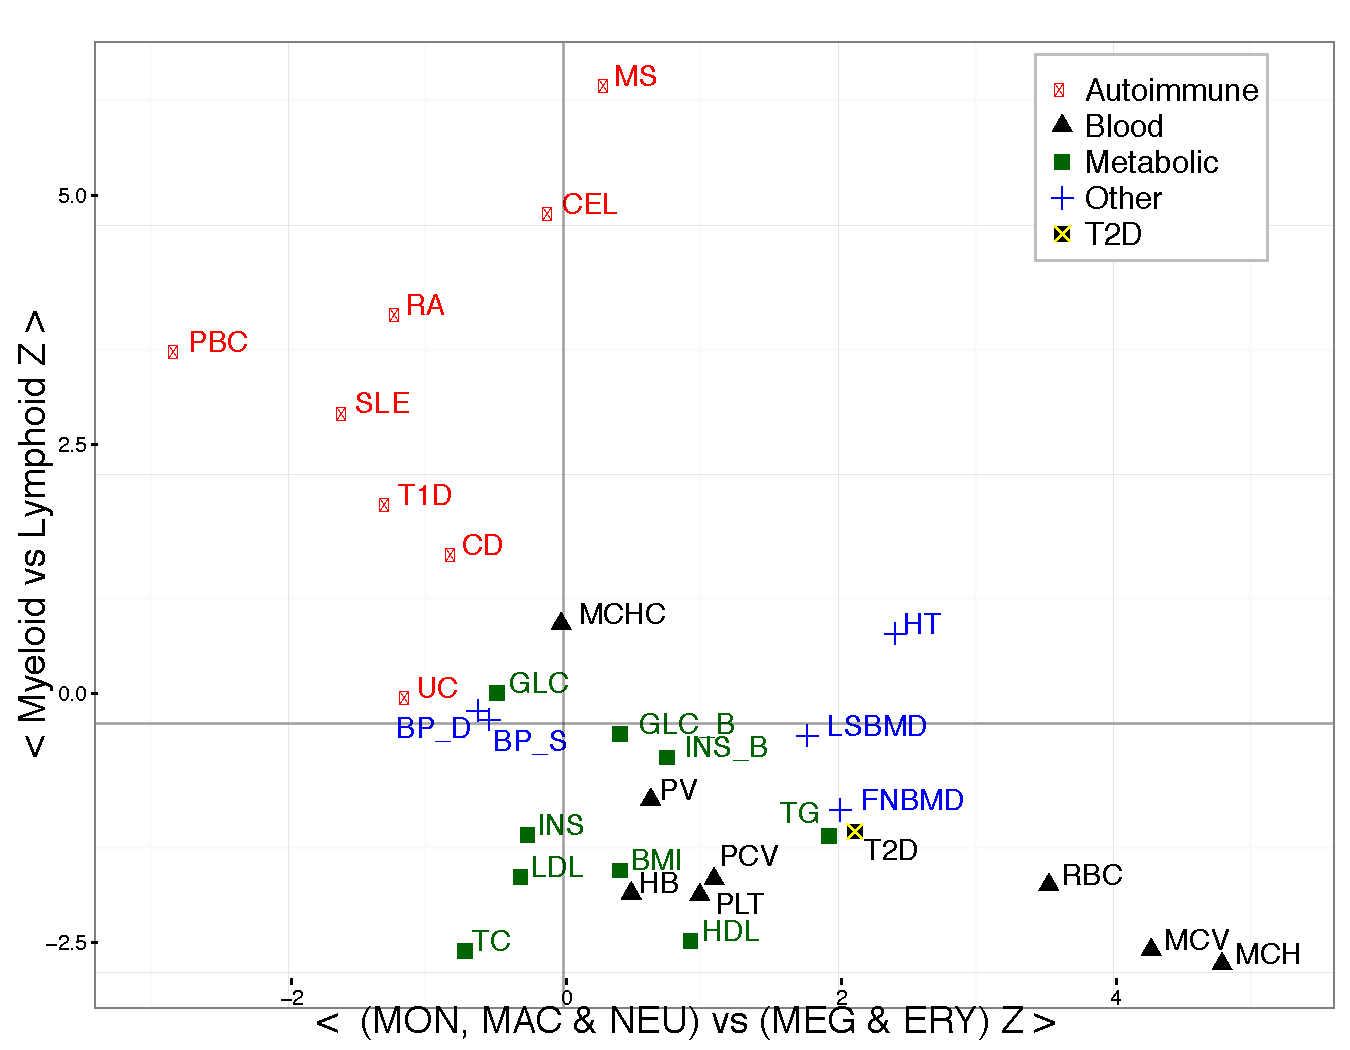
\includegraphics[width=0.7\textwidth]{block_shifter_scatter.pdf}
\caption{Enrichment of GWAS summary statistics at PIRs by tissue groups. Axes reflect \textit{blockshifter} $Z$-scores for two different tissue group comparisons, firstly lymphoid versus myeloid and then within myeloid lineage (MON - Monocyte, MAC - macrophage and NEU - Neutrophil) versus (MEG - Megakaryocyte and ERY - erythroblast). Traits are labelled and coloured by category (see appendix ?).}
\label{fig:bs_1}
\end{figure}

\begin{figure}[h]
\centering
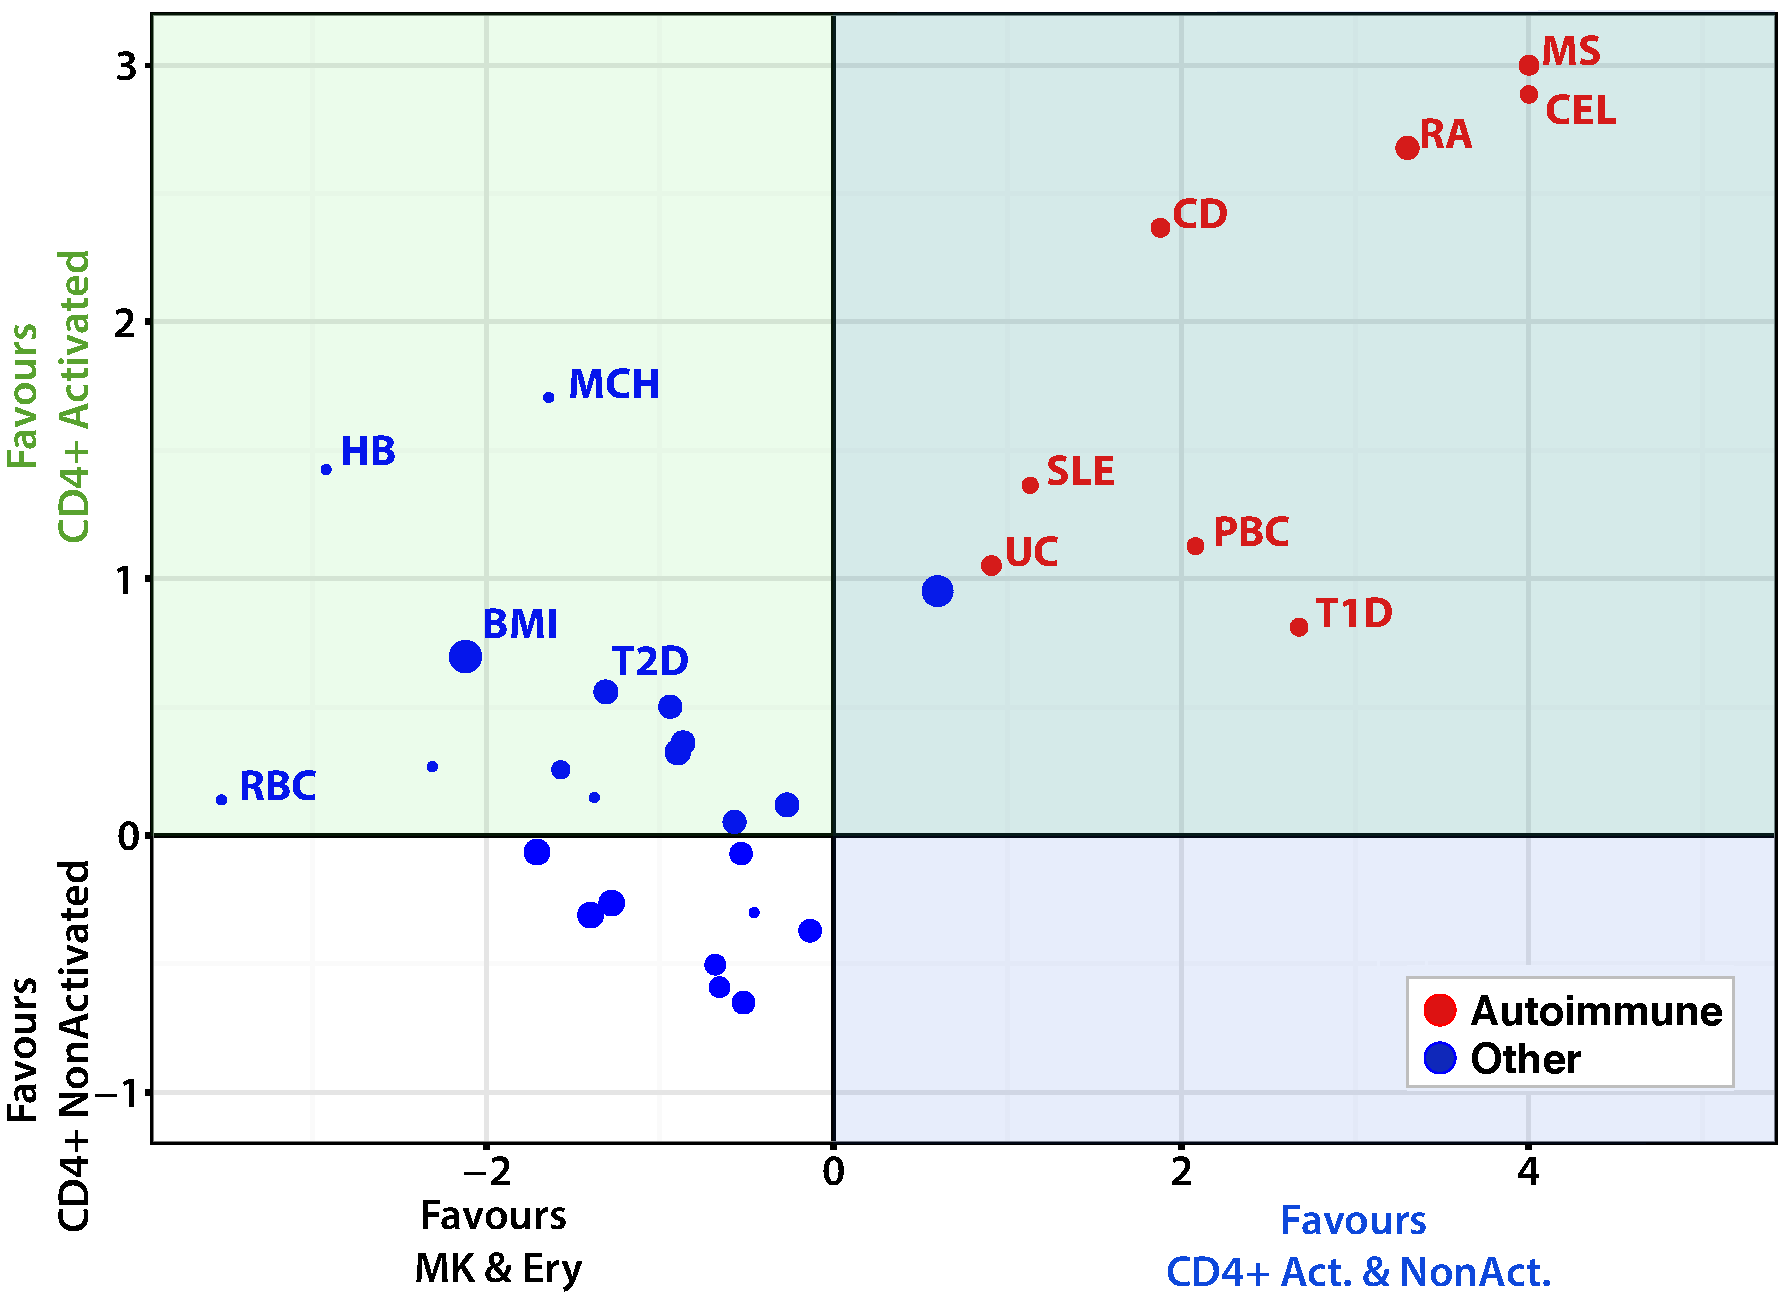
\includegraphics[width=0.7\textwidth]{tcell_blockshifter_scatter.pdf}
\caption{Tissue specific enrichment of autoimmune GWAS summary statistics at PIRs by tissue groups. Axes reflect \textit{blockshifter} $Z$-scores for two different tissue group comparisons, firstly MK - megakaryocytes and ERY - erythroblast versus Activated/Non-activated CD4$^{+}$ T cells. Y-axis shows comparison of Activated versus non activated CD4$^{+}$ T cells. Autoimmune traits are coloured red and other traits are blue, point size reflects the log transformed sample number included in each study.}
\label{fig:bs_2}
\end{figure}

\section{PCHiC assisted gene prioritisation across 31 traits}
 
Using COGS, I prioritised 2,604  unique protein coding genes (Overall COGS score $>$ 0.5) across all 31 traits examined. The prioritised genes exhibited enrichments for specific pathways in the Reactome pathway database~\citep{FabregatSidiropoulosGarapatiEtAl2016} in a naive analysis. As expected, genes prioritised for autoimmune diseases were enriched in inflammation and immune response-related pathways, such as interleukin and T cell receptor signalling, whereas genes prioritised for platelet traits were preferentially associated with platelet production and hemostasis (figure\ref{fig:reactome}). SNPs associated with traits generally unrelated to haematopoetic cells, such as blood pressure and bone mineral density did not show enrichment for PIRs in any of the cell types analysed.
%what are the stats for these prioritised genes ?

\begin{landscape}
\begin{figure}[p]
\centering
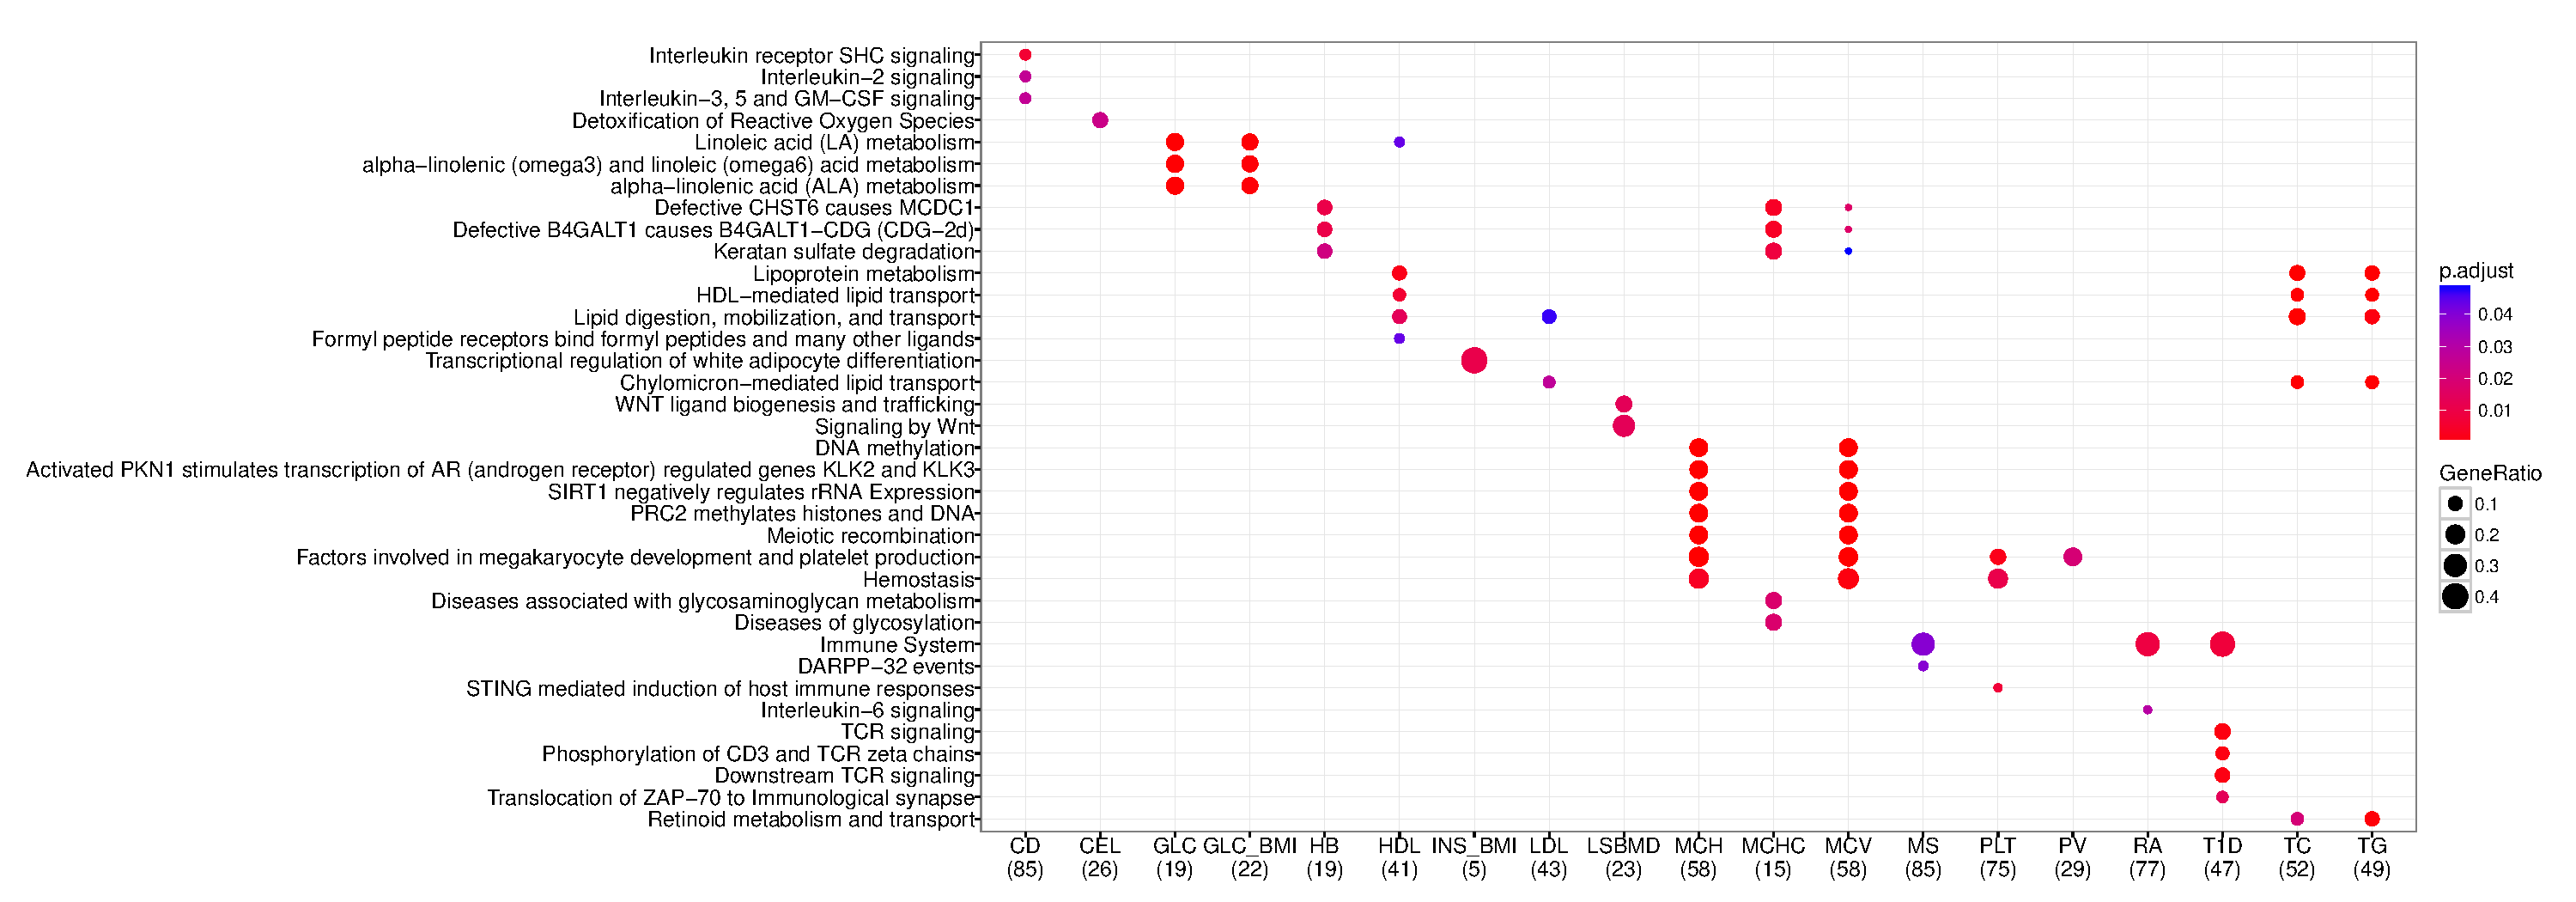
\includegraphics[scale=0.5]{hyper_reactome_analysis_2.pdf}
\caption{Bubble plot of traits with significant enrichment ($P_{adj} < 0.05$) in one or more reactome pathways  for genes with COGS score $>$ 0.5 across 31 traits. Number in parentheses below trait labels indicate the total number of genes analysed for each trait, bubble size indicates the ratio of test genes to those in the pathway, and blue to red shading corresponds to decreasing adjusted $P$-value for enrichment}
\label{fig:reactome}
\end{figure}
\end{landscape}



%In addition, the genes prioritised for RA included 5/9 candidates (C8Orf13, BLK, TRAF1, FADS2 and SYNGR1) that were identified in a recent study (Zhu et al., 2016) combining whole-blood eQTL with RA GWAS data by Mendelian randomisation. The relatively large number of prioritized genes without eQTL support is in agreement with previous reports of limited overlap of disease variants with eQTLs (Guo et al., 2015; Huang et al., 2015). This demonstrates complementary benefits of eQTL-based and physical interaction-based prioritization approaches for prioritizing identifying candidate target genes of non-coding disease variants.


%\section{Context specific gene priortisation across activated CD4$^{+}$ activated T cells}


\begin{figure}[h]
\centering
	 \begin{subfigure}{0.7\textwidth}
		%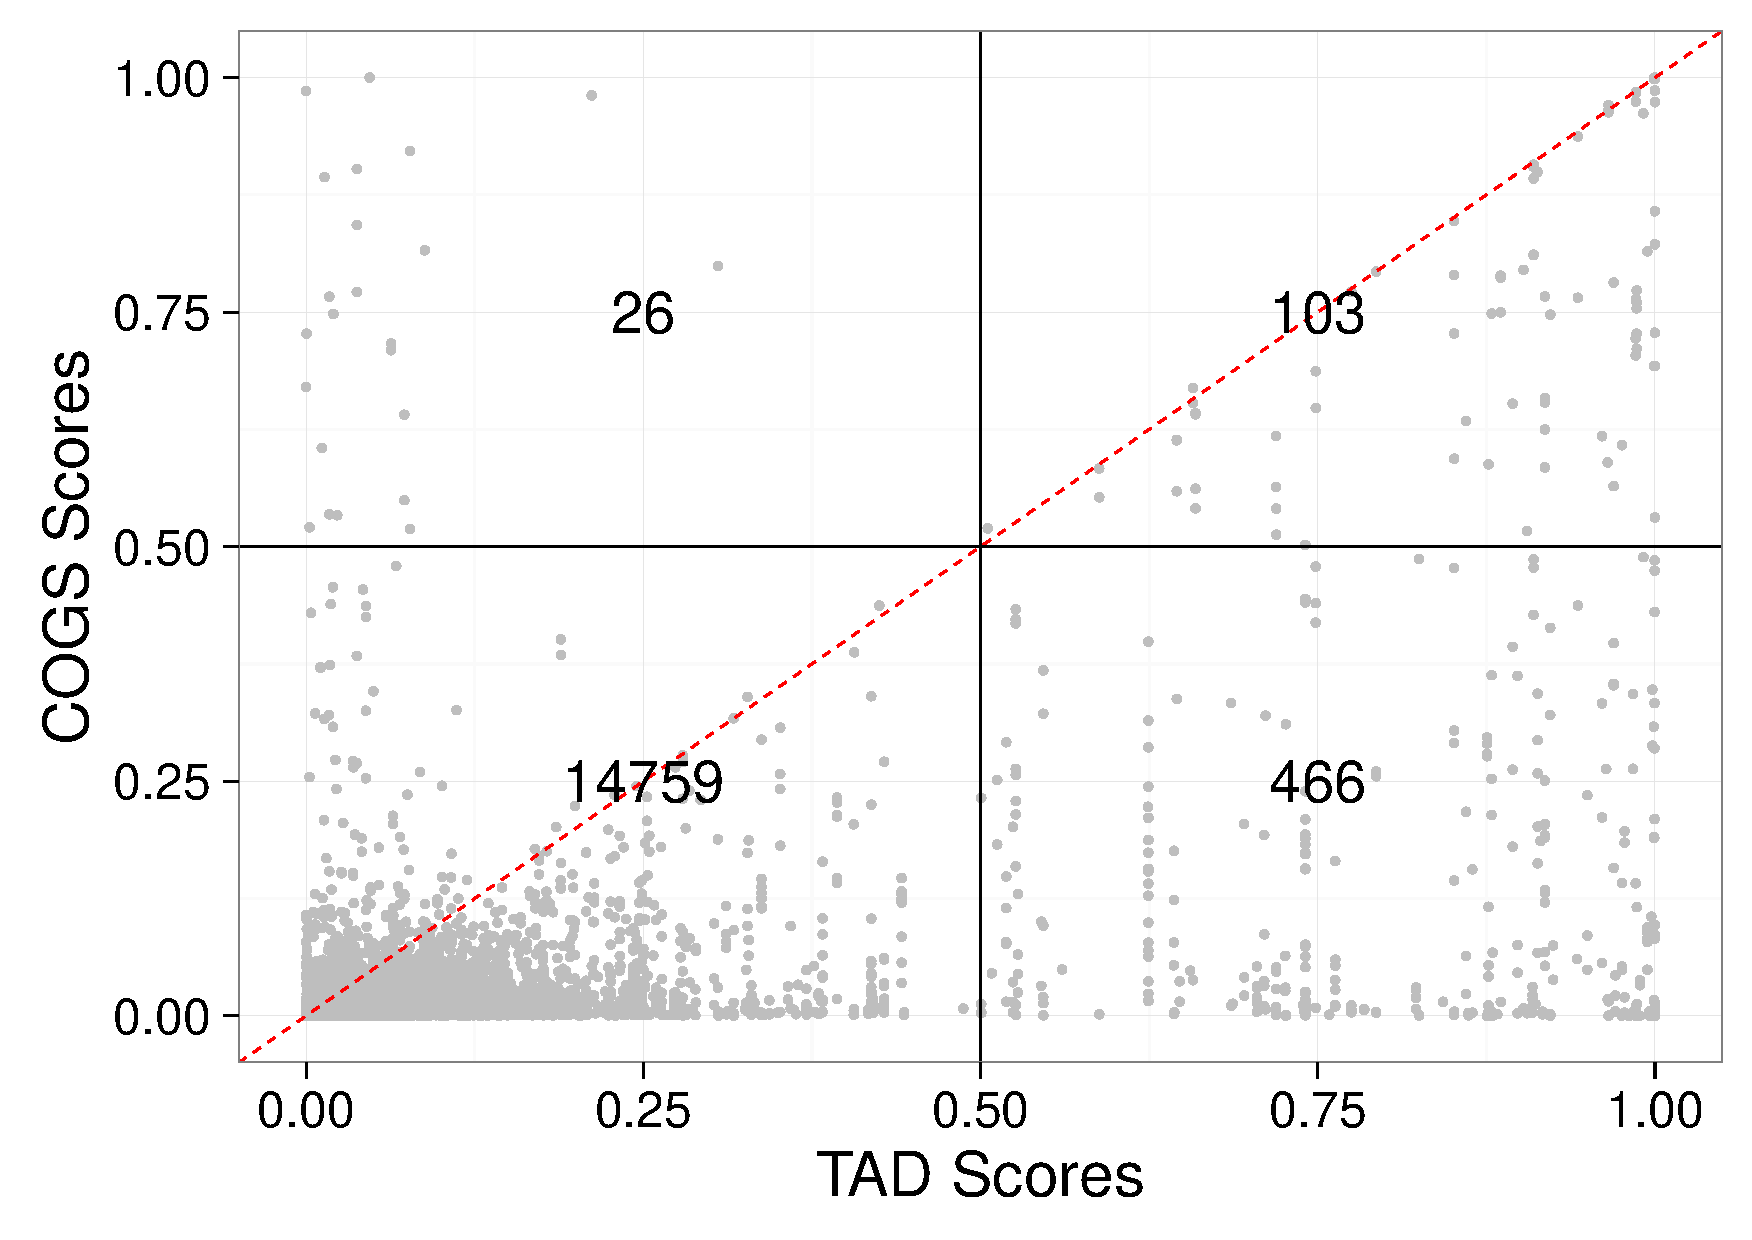
\includegraphics[width=\linewidth]{dot.pdf}
		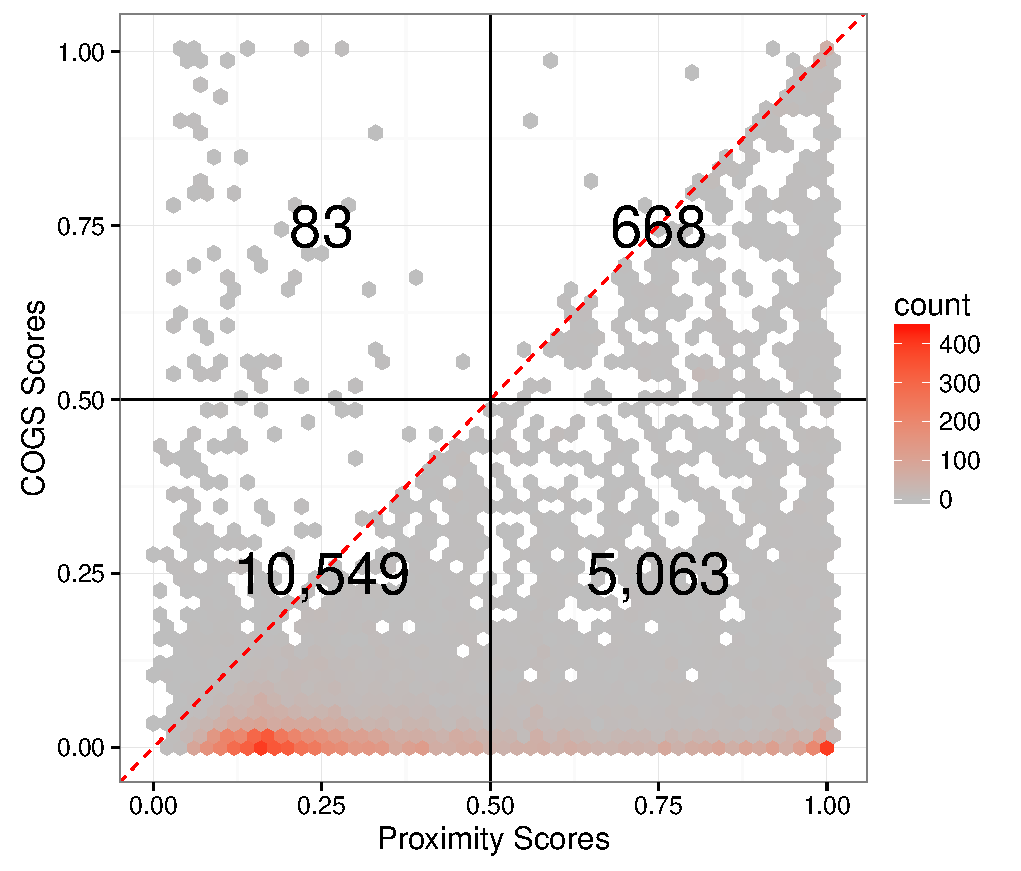
\includegraphics[width=\linewidth]{prox_compare.pdf}
		\caption{}\label{fig:fig_a}
	\end{subfigure}
	\hspace{1cm}
	\begin{subfigure}{0.7\textwidth}
		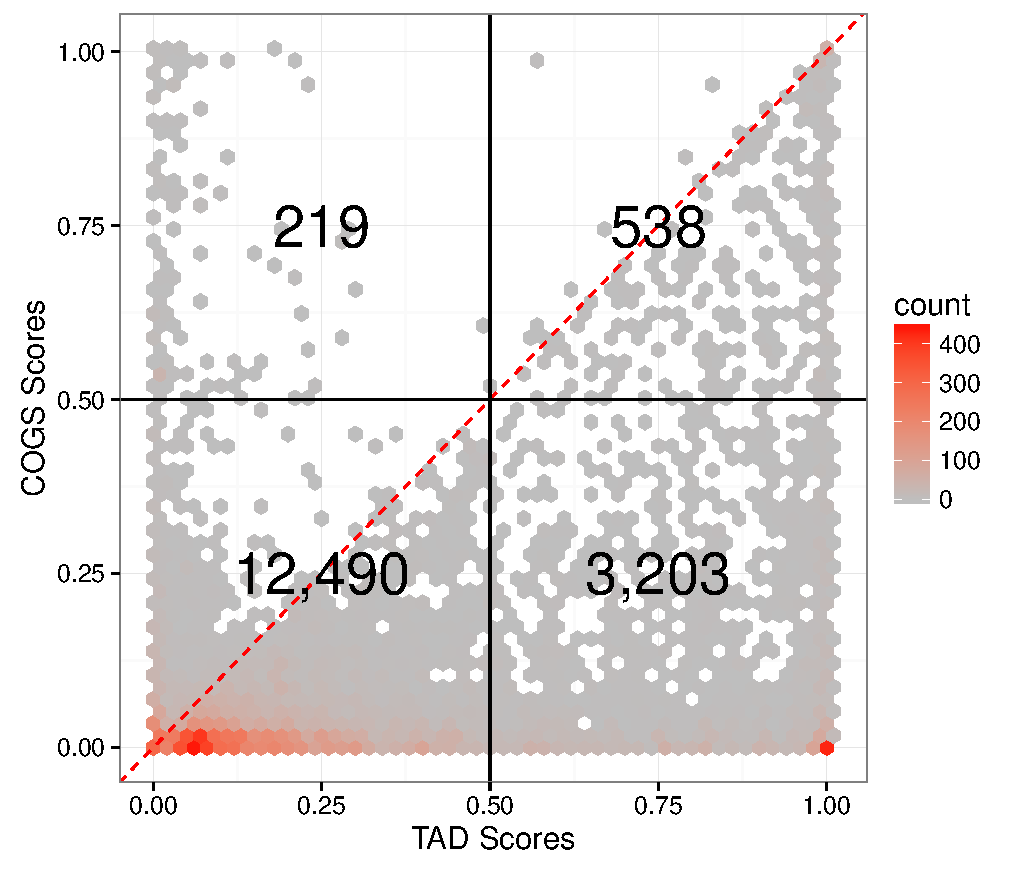
\includegraphics[width=\linewidth]{tad_compare.pdf}
		\caption{}\label{fig:fig_b}
	\end{subfigure}
\begin{minipage}[t]{0.7\textwidth}
	\caption{Comparison of autoimmune PCHi-C COGS scores and (\subref{fig:fig_a}) a proximity score from assigning variants to genes within 0.5 Mb of gene promoters (\subref{fig:fig_b}) Hi-C derived TAD scores, using 7 Cell types (Erythroblasts, Macrophages, Monocytes, Naive B cells, Naive CD4$^{+}$ T cells, Naive CD8$^{+}$ T cells and Neutrophils). Counts of genes in each quadrant are shown, grey to red colour gradient indicates gene density.}
\end{minipage}
\label{fig:cog_prox_comparison}
\end{figure}

\section{Prioritised genes do not overlap significantly with eQTLs}
In parallel with my GWAS focused analysis Oliver Stegle and Roman Kretzhuber (RK) had been working to consider expression quantative trail loci (eQTLs) from \citet{FairfaxMakinoRadhakrishnanEtAl2012} in the context of PCHi-C. Both eQTL and GWAS are enriched in PIRs, which prompted us to consider the overlap of COGS prioritised genes in SLE~\citep{Bentham2015-di} and rheumatoid arthritis~\citep{Okada2014-um} data sets, for which full imputed summary statistics were available. I performed COGS gene prioritisation and RK looked to see if there was evidence for overlap with relevant tissue eQTLs~\citep{FairfaxMakinoRadhakrishnanEtAl2012}.  Out of 456 genes that were prioritised for both traits 136 had eQTLs  of which four genes (\textit{BLK},\textit{RASGRP1}, \textit{SUOX}, and \textit{GIN1}) showed evidence for possible co-localization in RA and two genes (\textit{BLK} and \textit{SLC15A4}) in SLE. Additionally the genes prioritised for RA included 5/9 candidates (\textit{C8Orf13},\textit{BLK},\textit{TRAF1}, \textit{FADS2} and \textit{SYNGR1}) that were identified in a recent study~\citep{ZhuZhangHuEtAl2016} that combined whole blood eQTLs with the same RA GWAS data by Mendelian randomisation. The relatively large number of GWAS prioritised genes without eQTL support  agrees with previous reports of limited overlap of disease variants with eQTLs~\citep{Guo2015-ka,HuangChenEsparzaEtAl2015}. One reason for this observation might be that the causal variant functions in a specific tissue context and thus it's eQTL is not observable in available eQTL datasets. The implication of this is that regulatory annotations that might be used to augment fine mapping methods are similarly incomplete. 

\section{COGS prioritisation qualitatively performs better than TAD and distance based scores}
For all eight GWAS autoimmune traits, I compared protein coding genes scores, using PCHiC datasets (COGS), and comparitive scores computed using TAD and proximal methods. To summarise results across all diseases I selected the maximum score for a method for each gene. Using a score cut off of 0.5 I then categorised each gene as to whether it was prioritised in either a single, both or no methods (Figure \ref{fig:cog_prox_comparison}). In general COGS prioritised genes sets were significantly smaller than then those from the other methods. The naive proximity based score appeared to be least specific prioritising 5,731 genes in total, however it had the greatest overlap with COGS scores implying comparatively better sensitivity. For proximity based scores 83 genes were prioritised exclusively by COGS, indicating that 12\% of genes are prioritised by interactions greater than 0.5 Mb. TAD based scores 219 genes were prioritised exclusively by COGS, indicating that approximately 30\% of genes are prioritised by interactions that span TAD boundaries.  I note however that examining distance metrics between gene baits and supporting PIRs that in some cases this could be due to the imprecise definition of TAD boundaries (Figure \ref{fig:distance_distro}). Overall COGS appears to select genes not found by other methods and also appears to be more specific.

\begin{figure}[h]
\centering
	 \begin{subfigure}{0.7\textwidth}
		%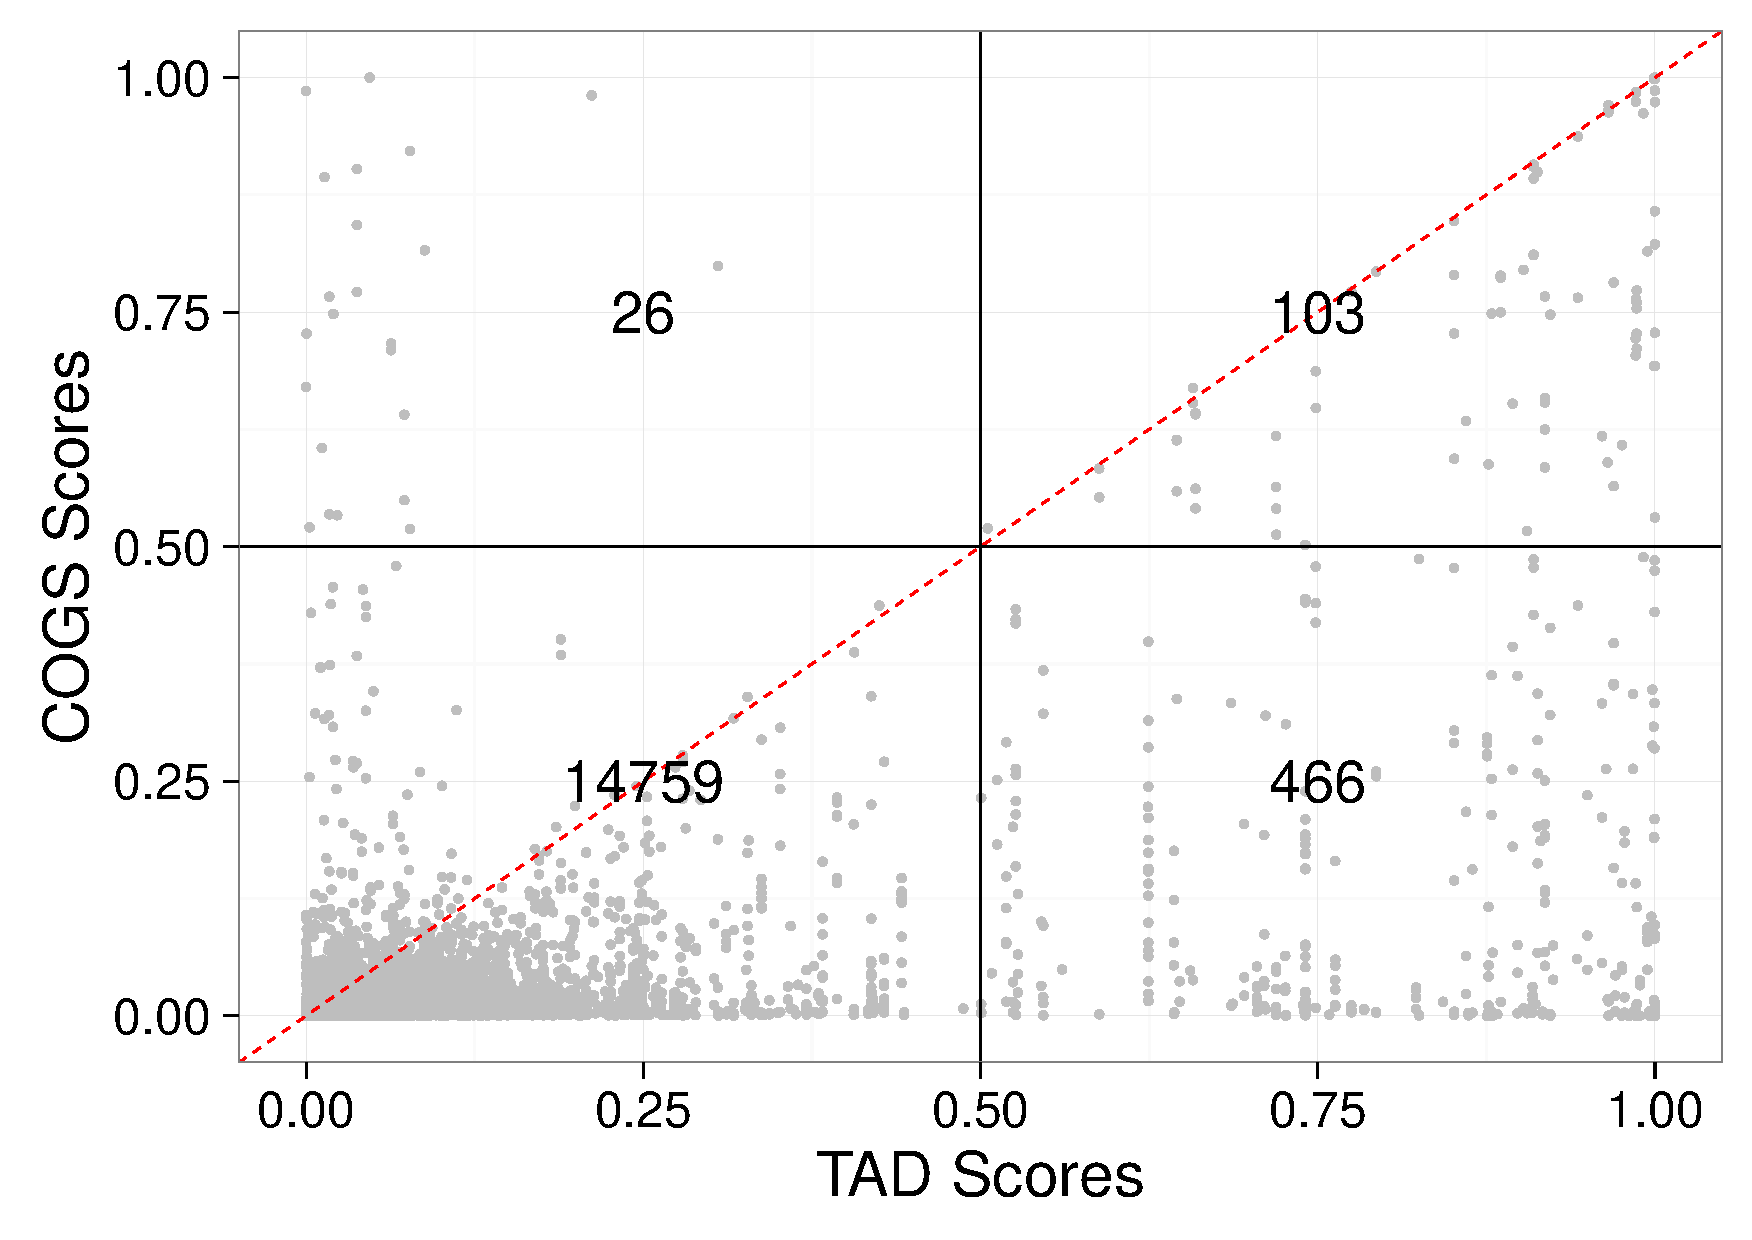
\includegraphics[width=\linewidth]{dot.pdf}
		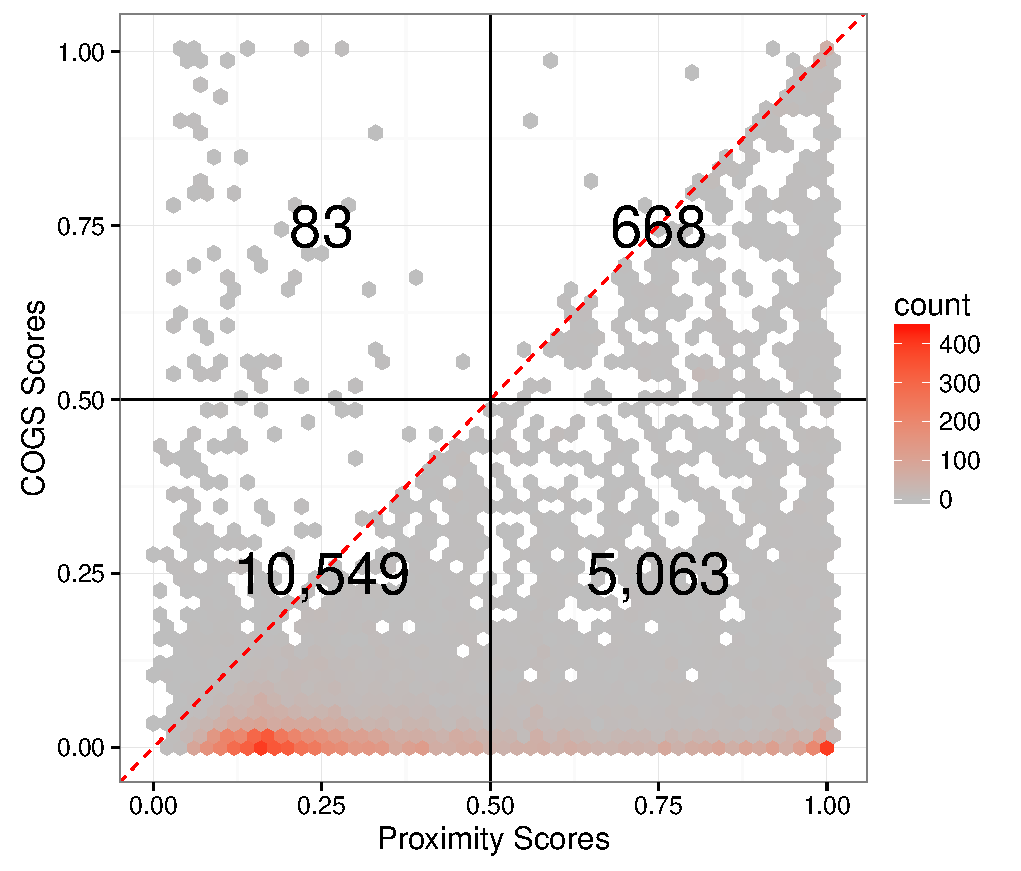
\includegraphics[width=\linewidth]{prox_compare.pdf}
		\caption{}\label{fig:fig_a}
	\end{subfigure}
	\hspace{1cm}
	\begin{subfigure}{0.7\textwidth}
		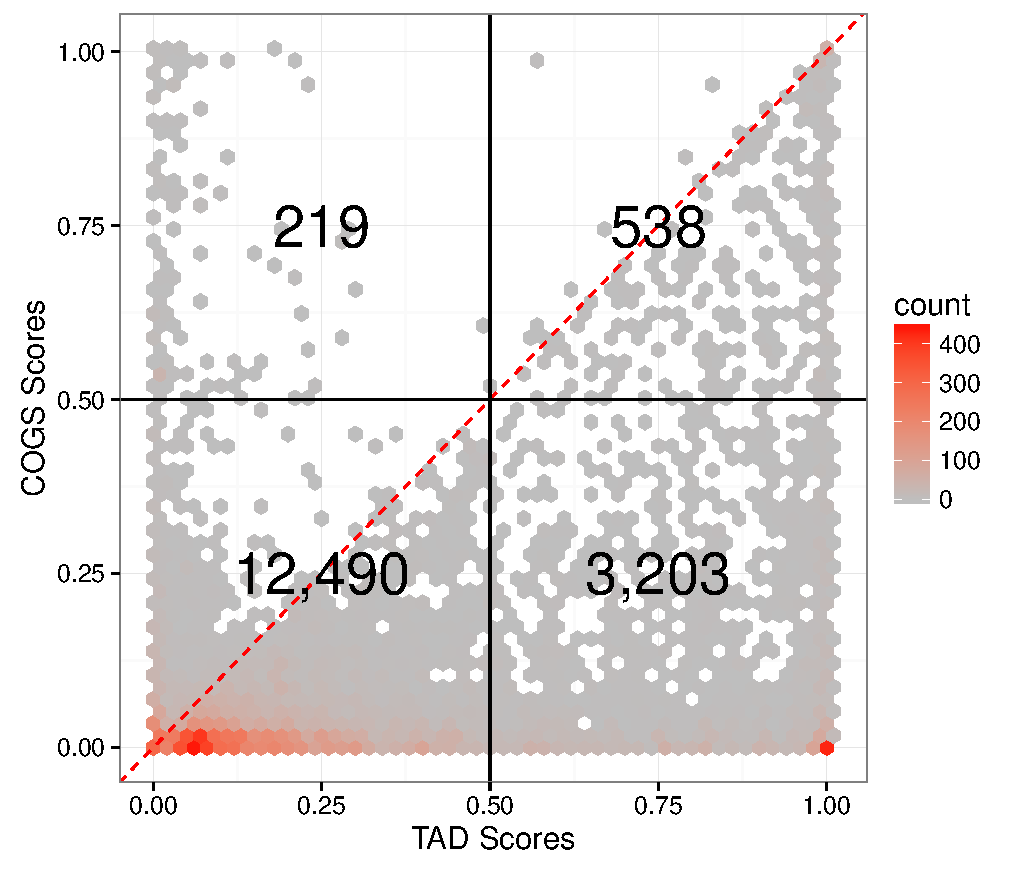
\includegraphics[width=\linewidth]{tad_compare.pdf}
		\caption{}\label{fig:fig_b}
	\end{subfigure}
\begin{minipage}[t]{0.7\textwidth}
	\caption{Comparison of autoimmune PCHi-C COGS scores and (\subref{fig:fig_a}) a proximity score from assigning variants to genes within 0.5 Mb of gene promoters (\subref{fig:fig_b}) Hi-C derived TAD scores, using 7 Cell types (Erythroblasts, Macrophages, Monocytes, Naive B cells, Naive CD4$^{+}$ T cells, Naive CD8$^{+}$ T cells and Neutrophils). Counts of genes in each quadrant are shown, grey to red colour gradient indicates gene density.}
\end{minipage}
\label{fig:cog_prox_comparison}
\end{figure} 

\begin{figure}[ht]
\centering
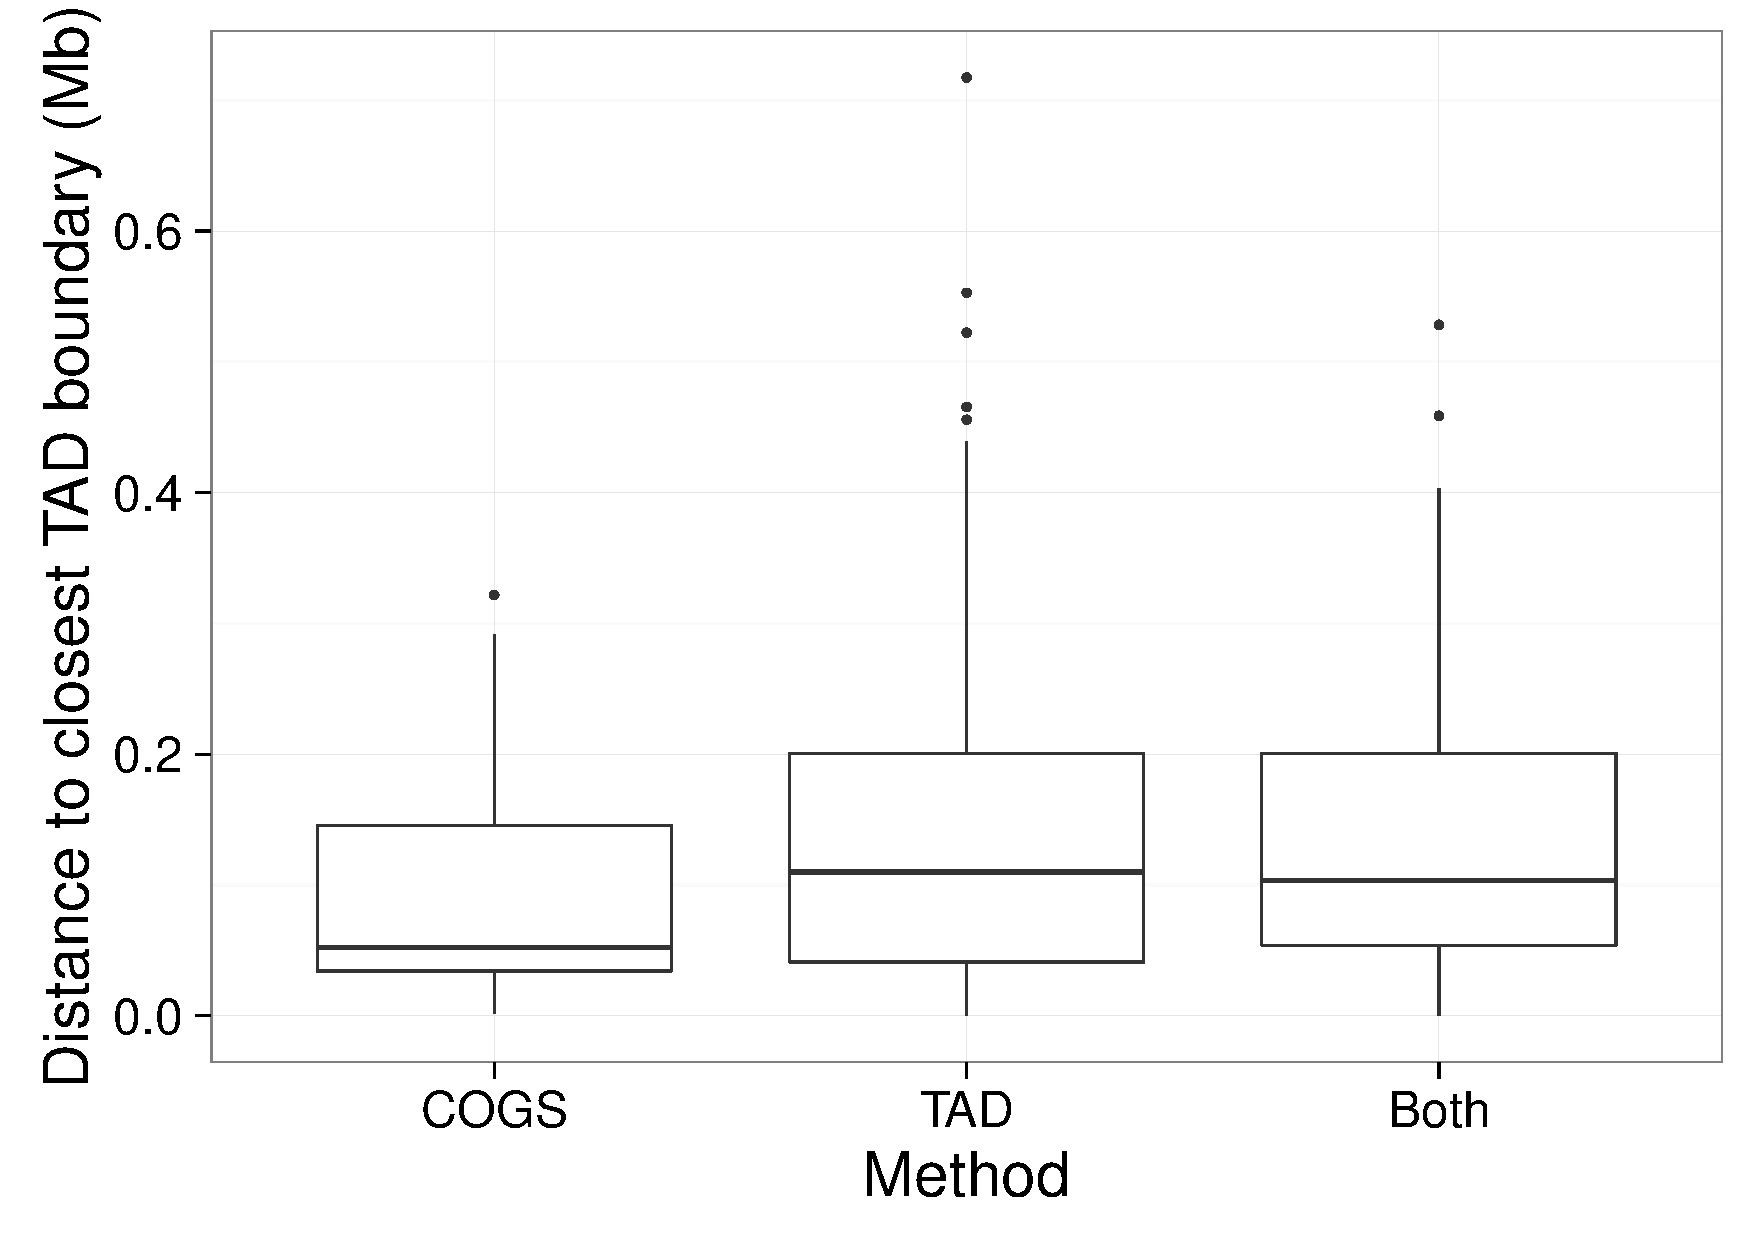
\includegraphics[width=0.7\textwidth]{dist_boxplot.pdf}
\caption{Box plot showing the distribution of distances between baits and TAD boundaries for significant (score $>$ 0.5) genes. ’Both’ indicates that gene was significant using TAD and COGS methods}
\label{fig:distance_distro}
\end{figure}

\section{COGS prioritised genes are enriched for disease specific differentially expressed genes} 
Calibrating performance metrics of the COGS method is challenging in the absence of a test set of scores, one possible proxy is to examine the overlap of prioritised genes with studies examining differential expression between diseased and healthy volunteers in relevant tissue types. I integrated scores from PCHi-C (COGS), proximity and TAD methods, for ulcerative colitis (UC) and Crohn's disease (CD), with differentially expressed genes (FDR 5\%) from~\citet{PetersLyonsLeeEtAl2016} and used Fishers Test to examine enrichment for prioritised genes (score $>$ 0.5). I found that UC COGS genes were significantly enriched for differentially expressed genes ($P = 0.002$), for Crohn's disease there was nominal enrichment ($P = 0.04$). Conversely there was no evidence of enrichment in any datasets using proximal and TAD methods (Figure \ref{fig:peters_odds_ratio}). The intersect between differentially expressed genes and COGS prioritised genes indentified 67 genes (Table \ref{tab:ibd_genes}). Whilst there are many candidate genes in this list, an example on chromosome 3 for ulcerative colitis provides an illustration of the potential for hypothesis generation by integrative analysis of PCHi-C interaction maps (Figure \ref{fig:bcl6}). COGS prioritises \textit{BCL6} gene which has been shown to have potent effects on Th9 cell development and IL-9 secretion both important modulators of inflammation~\citep{BassilOrentOlahEtAl2014}. Putative causal variants from~\citet{Anderson2011-ch} reside in intron 8 of \textit{LPP}, and previous studies have inferred this gene as responsible for, however PCHi-C results from lymphoid tissues show interactions between this region and the \textit{BCL6} promoter. Furthermore, BLUEPRINT chromatin state maps classify this region harbouring putatitive causal variants as having enhancer activity across 3 out of 4 biological replicates in CD4$^+$ T cells. Expression profiles from~\citet{PetersLyonsLeeEtAl2016} show that whilst LPP is not significantly differentially expressed between UC controls and healthy volunteers($\log(\text{Fold Change})$ = 0.05, $P_{adj}$ =  0.46) \textit{BCL6} ($\log(\text{Fold Change})$ = 0.22, $P_{adj}$ =  0.0018), providing further support for it's prioritisation.

\begin{figure}[ht]
\centering
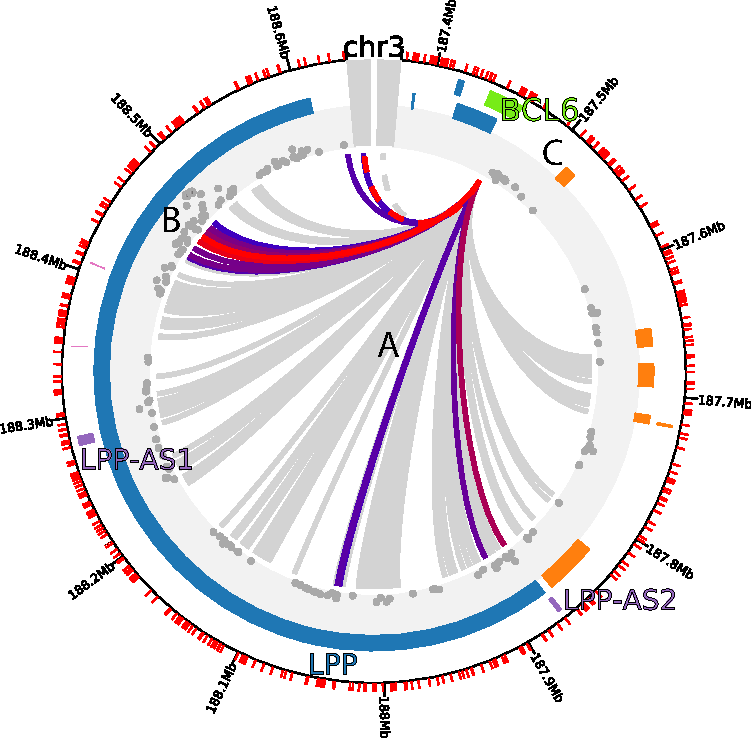
\includegraphics[width=0.7\textwidth]{CHiCP-BCL6-Naive_CD4.pdf}
\caption{Circularised plot showing overlap between ulcerative colitis (UC) putative variants and  interactions between \textit{BCL6} gene promoter in CD4$^+$ T cells, prioritised by COGS algorithm. A) Interactions, grey (not significant (CHiCAGO score $<$ 5 but significant in other tissues), blue (less significant) to red(more significant) colour gradient. B) UC GWAS summary $-\log(P)$ values from~\citet{Anderson2011-ch} C)  Gene annotations, protein coding (blue), antisense (purple), lincRNA (orange) and \textit{BCL6} (green). Red ticks around circumference indicate \textit{Hind}III fragament boundaries. Figure modified from CHiCP - \url{http://www.chicp.org}~\citep{SchofieldCarverAchuthanEtAl2016} }
\label{fig:bcl6}
\end{figure}

\begin{figure}[ht]
\centering
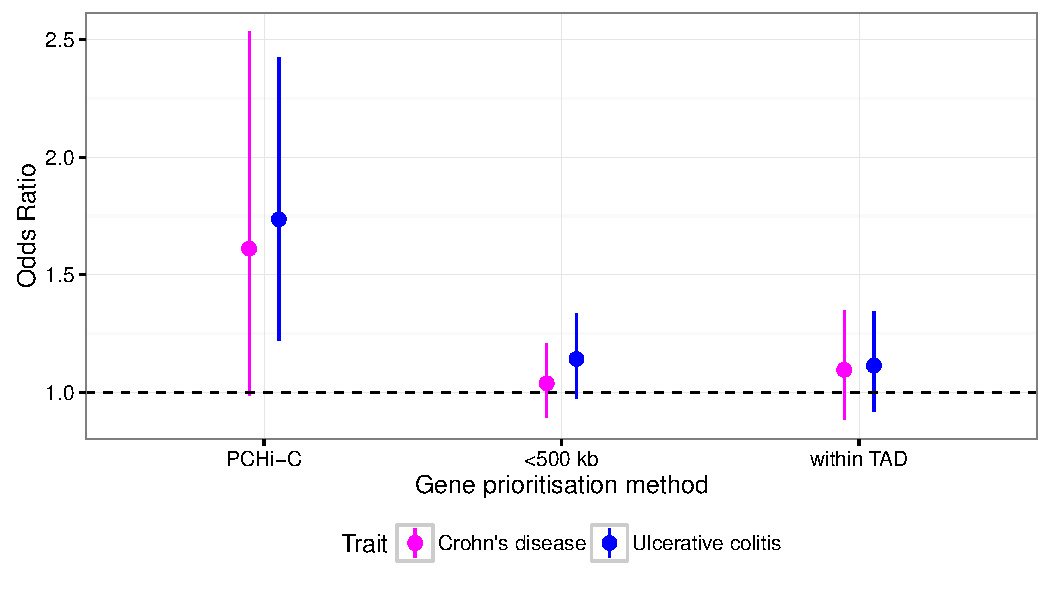
\includegraphics[width=0.7\textwidth]{ibd-tadprox.pdf}
\caption{Enrichment of prioritised genes in ulcerative colitis and Crohn's differentially expressed genes from~\citet{PetersLyonsLeeEtAl2016}. Methods PCHi-C (COGS), $<$ 500 Kb (Proximity) and within TAD (topologically associated domain).}
\label{fig:peters_odds_ratio}
\end{figure}

\section{Tissue specific PCHiC assisted gene prioritisation using dense summary statistics}
The stronger enrichment of autoimmune disease GWAS traits in activated CD4$^+$ T cells lead us to examining autoimmune traits in the context of activated and non activated CD4$^{+}$ promoter interaction maps. We extended COGs to  incorporate a simple binary decision tree model to allow tissue or functional category resolution (see methods).  Across the combined GWAS and ImmunoChip autoimmune data sets I was able prioritise 602 distinct protein coding genes  (Figure\ref{fig:cogs_ai}). To summarise the behaviour of prioritisation, I focused on a subset of 220 input autoimmune GWAS regions with genome-wide significant signals ($P<5 \times 10^{-8}$). I prioritised at least one gene with a COGS scores $>0.5$ in 122 of these regions, with a median of two genes/region (inter quartile range = 1-3). The average distance from peak signal to prioritised genes was 334 kb and I observed a median of three genes `skipped' between GWAS signal peaks and prioritised genes. Using pooled total RNA-seq expression data on the same donors (Anthony Cutler, Arcadio Rubio Garcia and Chris Wallace), I found that 457 of the prioritised genes were expressed in at least one activation state. I could relate 259 genes to GWAS significant signals of which 166 were deferentially expressed between activated and non activated states.

\section{Allowing multiple causal variants increases number of prioritised genes}
I wanted to understand the effect of assuming a single causal variant within each region on gene COGS scores for various traits. I compared COGS scores computed from marginal posterior probabilites for dense genotype data from four autoimmune diseases (ATD, CEL, RA and T1D) , computed by GUESS FM, which allow multiple causal variants to those from PMI, which assumes a single common variant (figure \ref{fig:gfm_vs_pmi_gs}). Generally there is agreement between imethods, however I note that in general GUESSFM prioritses more genes than PMI (Table \ref{tab:cogs_gfm_pmi}). This increase in specificity may be down to increased resolution gained from the GUESSFM approach due to the employment of genotype based imputation and it's ability to consider different prior probabilities. Some of this will be offset by a greater sensitivity to genotyping error than the PMI based approach.

\begin{table}[ht]
\centering
\begin{tabular}{lrrrr}
  \hline
Disease & GUESSFM & PMI & Both & Total \\ 
  \hline
ATD &   9 &   0 &   6 &  38 \\ 
CEL &   6 &   5 &  33 & 114 \\
RA &   6 &   2 &  19 & 132 \\ 
T1D &  16 &   7 &  35 & 212 \\ 
\hline
\end{tabular}
\label{tab:cogs_gfm_pmi}
\caption{Counts for protein coding genes prioritised (score $>$ 0.5) by GUESSFM, Poor Man's Imputation (PMI) and Both methods out of Total genes with score $>$ 0.01.} 
\end{table} 

%\section{Gene set enrichment analysis of COGS prioritised genes using MSigDB HALLMARK gene sets} 

%To check whether the list of prioritised genes corresponded to existing biological understanding of autoimmune disease, in collaboration with Chris Wallace we used gene set enrichment analysis of the genome wide COGS scores as described in the methods  across 31 traits to MSigDB HALLMARK gene sets. We found significantly greater (Bonferroni $p<0.05$) enrichment in autoimmune diseases compared to non-autoimmune traits in four gene sets relating to signalling and receptor molecules as well as reactive oxygen species involved in early T cell activation (figure \ref{fig:hallmark}).

\begin{figure}[h]
\centering
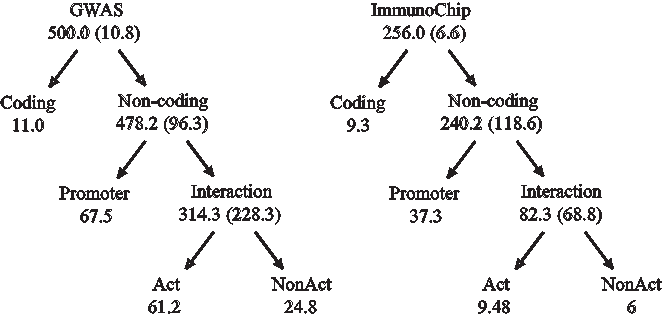
\includegraphics[width=0.7\textwidth]{ai_cogs.pdf}
\caption{Functional gene prioritisation across 11 autoimmune diseases using genome wide (GWAS) or targeted genotyping array (ImmunoChip) data. The numbers at each node give the number of genes prioritised at that level. Where there is evidence to split into one of two non-overlapping hypotheses ($\log_{10}$ ratio of gene scores $>$3), the genes cascade down the tree. Where the evidence does not confidently predict which of the the two possibilities is more likely, genes are `stuck' at the parent node (number given in brackets). When the same gene is prioritised for multiple ($n>1$) disease, we assigned a fractional count to each node, defined as the proportion of the $n$ disease for which the gene was prioritised at that node.}
\label{fig:cogs_ai}
\end{figure}

%\begin{figure}[h]
%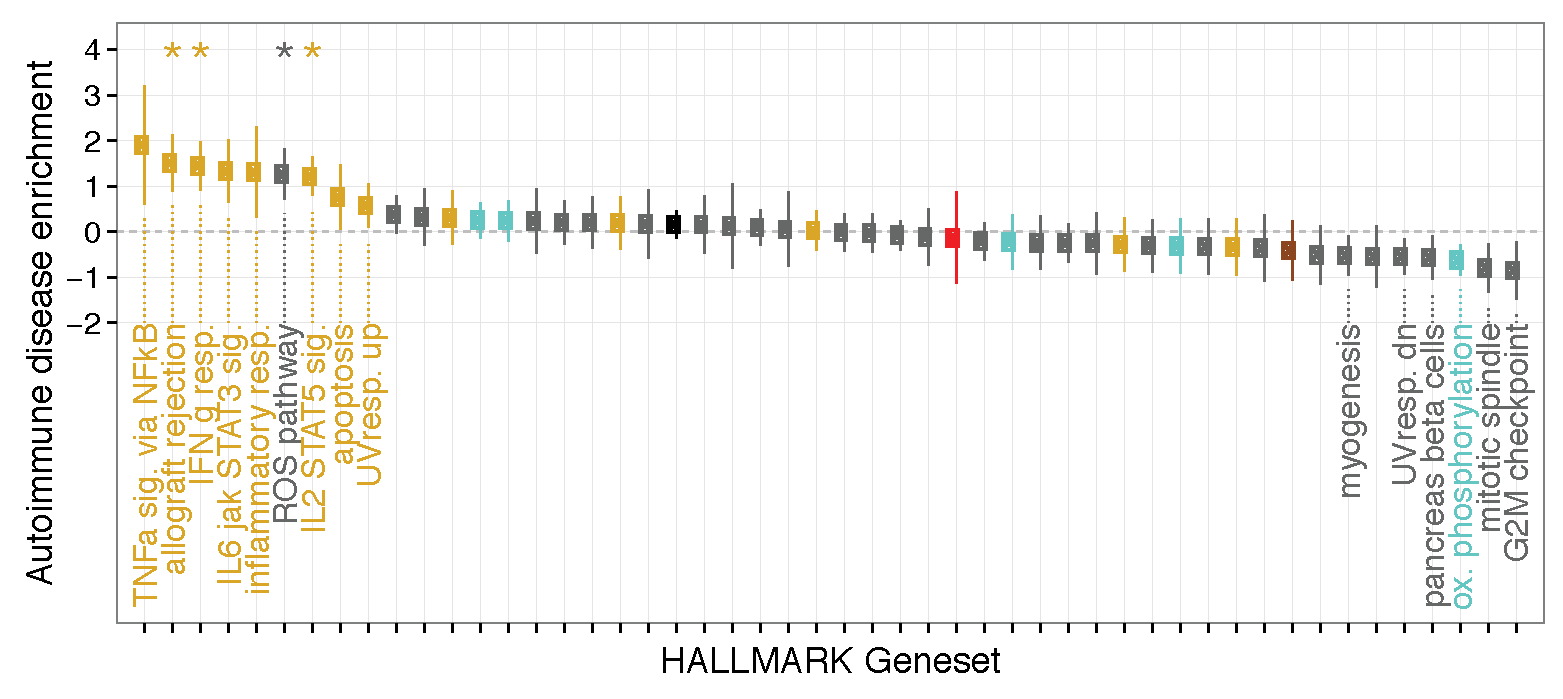
\includegraphics[width=\textwidth]{hallmark_enrichment.pdf}
%\caption{Tissue specific gene set enrichment analysis using COGS gene prioritisation scores for 11 autoimmune traits. Colours correspond to shared pathways enriched in modules identified by weighted gene correlation network %analysis (WGCNA) of activated vs non-activated CD4$^{+}$ T cells RNA-Seq data. Points give the difference in average enrichment of $Z$ scores across autoimmune versus non-autoimmune GWAS and bars the 95$\%$ confidence interval. Significant gene sets after Bonferroni correction are indicated by $*$.}
%\label{fig:hallmark} 
%\end{figure}

\begin{figure}[h]
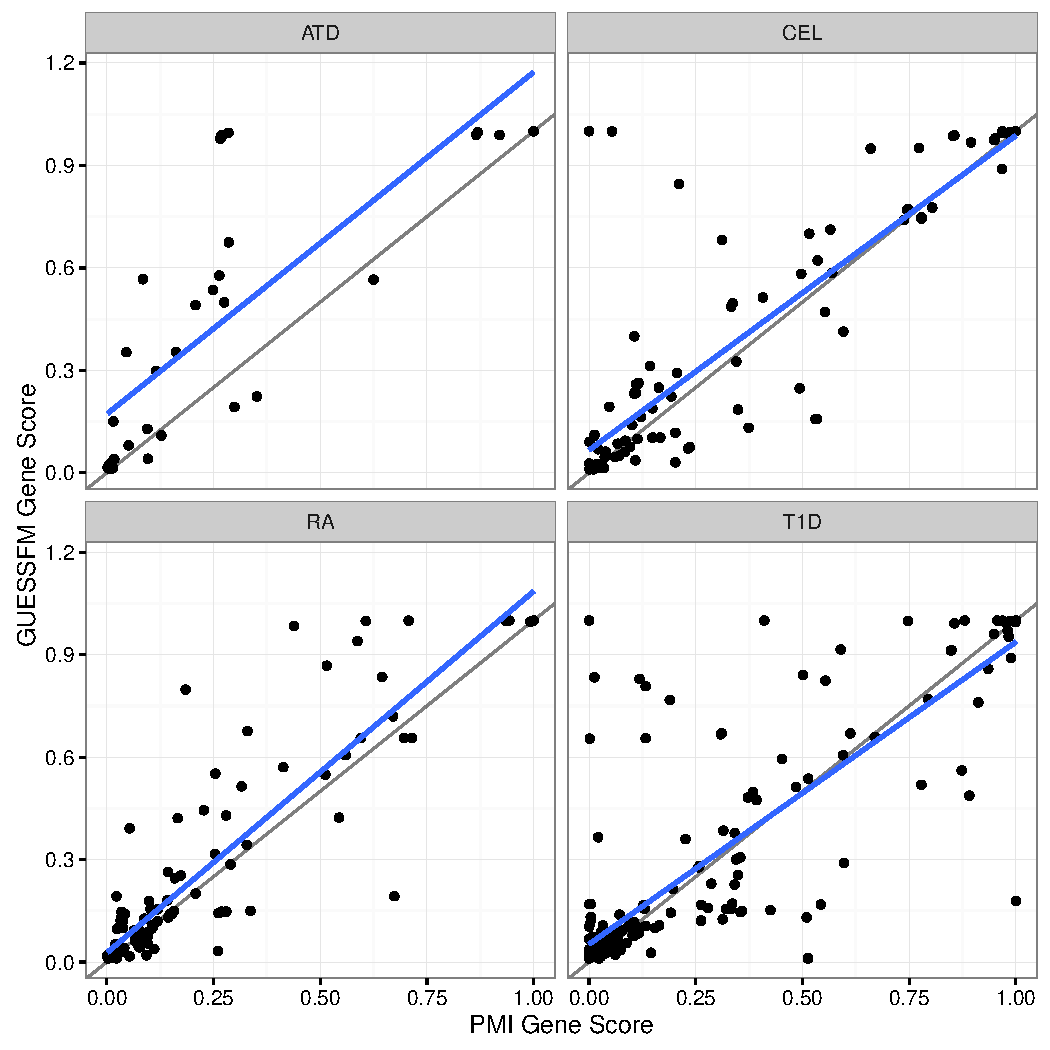
\includegraphics[width=\textwidth]{gfm_vs_pmi_gs.pdf}
\caption{Comparison of COGS gene scores for four autoimmune traits (ATD = autoimmune thyroid disease, CEL = celiac disease, RA = rheumatoid arthritis and T1D = type 1 diabetes computed using marginal posteriors from GUESSFM method and those computed using posteriors from PMI, grey line shows $y=x$, blue lines indicate the fitting of a linear model}
\label{fig:gfm_vs_pmi_gs}
\end{figure}ß


%\section{CHiCP: a genome browser for PCHiC interaction maps}
%In collaboration with Ellen Schofield, I developed a web based application, CHiCP \url{https://www.chicp.org}, to allow the visual integration of both public and private promoter capture Hi-C maps with GWAS and BLUEPRINT epigenetic data~\citep{SchofieldCarverAchuthanEtAl2016}. To do this I developed an interactive circularised display, with a search interface  for genes, variants and chromosomal coordinates. An interaction can be selected, allowing users to access a conventional browser view to see a zoomed in view of chromatin states and GWAS signals at promoter and promoter interacting regions.

\chapter{Discussion}

I have presented \textit{in silico} validation for genes prioritised by integrating PCHi-C and GWAS datasets. In collaboration with Daniel Rainbow, Tony Cutler, Arcadio Rubio Garcia, Chris Wallace and Linda Wicker we sought to understand how we might functionally validate one such prioritised gene and whether this might lead to a greater understanding of how causal variation might modulate autoimmune disease susceptibility.
%\section{Summary} %prerhaps goes at the end ?
%Methods to integrate genetic and genomic data sets are important in order to identify causal variants, genes and pathways and the tissue contexts within which they operate. I have developed two Bayesian approaches to integrate GWAS summary statistics and targeted genotyping data (ImmunoChip) with high resolution chromatin conformation data. Firstly \textit{blockshifter}, a method to perform competitive tissue enrichment analysis in the presence of correlation in order to prioritise relevant tissue contexts. Secondly COGS, a method to prioritise causal candidate genes based across tissue contexts and traits.  I used \textit{blockshifter} to verify the relevance of chromatin interactions with activated and unactivated CD4$^{+}$ T cells to autoimmune traits. Using COGS I was able to prioritise a number of genes for further study, I performed gene set analysis using a standard hypergeometric method on the Reactome database and a tissue specific GSEA using MolSigDB HALLMARK gene sets which indicated that COGS prioritised genes  were enriched for both expected and unexpected pathways. 

\section{Functional validation of COGS prioritised gene \textit{IL2RA}}
I have presented \textit{in silico} validation for genes prioritised by integrating PCHi-C and GWAS datasets. In collaboration with Daniel Rainbow, Tony Cutler, Arcadio Rubio Garcia, Chris Wallace and Linda Wicker we sought to understand how we might functionally validate one such prioritised gene and whether this might lead to a greater understanding of how causal variation might modulate autoimmune disease susceptibility. COGS analysis prioritised, in multiple diseases (autoimmune thyroid disease, Crohn's disease, multiple sclerosis, rheumatoid arthritis, type 1 diabetes, and ulcerative colitis) \textit{IL2RA} which encodes the CD25 protein which is a component of the IL-2 receptor that is essential for high-affinity binding of IL-2, regulatory T cell survival and T effector cell differentiation and function~\citep{LiaoLinLeonard2013}. I found this prioritisation to be driven by an interaction between the IL2RA promoter and a PIR in exon 1 known to harbour a set of type 1 diabetes putative causal SNPs (Figure\ref{fig:il2ra_ase_region}) identified in a previous fine mapping study~\citep{WallaceCutlerPontikosEtAl2015}. This  set of SNPs(Figure\ref{fig:il2ra_ase}a) is in high LD ($r^{2} > 0.8$) with rs12722495 which has been shown to affect the surface expression CD25 in memory T cells~\citep{DendrouPlagnolFungEtAl2009}. Using a targeted RNA-sequencing approach, and software I helped to develop previously~\citep{RainbowYangBurrenEtAl2015} Daniel Rainbow measured the relative expression of the two alleles at one of these set `A' SNPs, rs61839660, in intronic cDNA from four individuals heterozygous at rs61839660 and homozygous across most other associated SNP groups, in a four-hour activation time-course of CD4$^{+}$ T cells. We observed allelic imbalance in non activated CD4$^{+}$ T cells however on activation this was lost suggesting a context specific effect within this locus. To ensure this reflected imbalance in transcription of \textit{IL2RA}, and not simply enhancer RNAs in intron 1,  further validation was performed using rs12244380 found in the 3' UTR of \textit{IL2RA} (Figure\ref{fig:il2ra_ase_tc}). 

\begin{figure}[h]
\centering
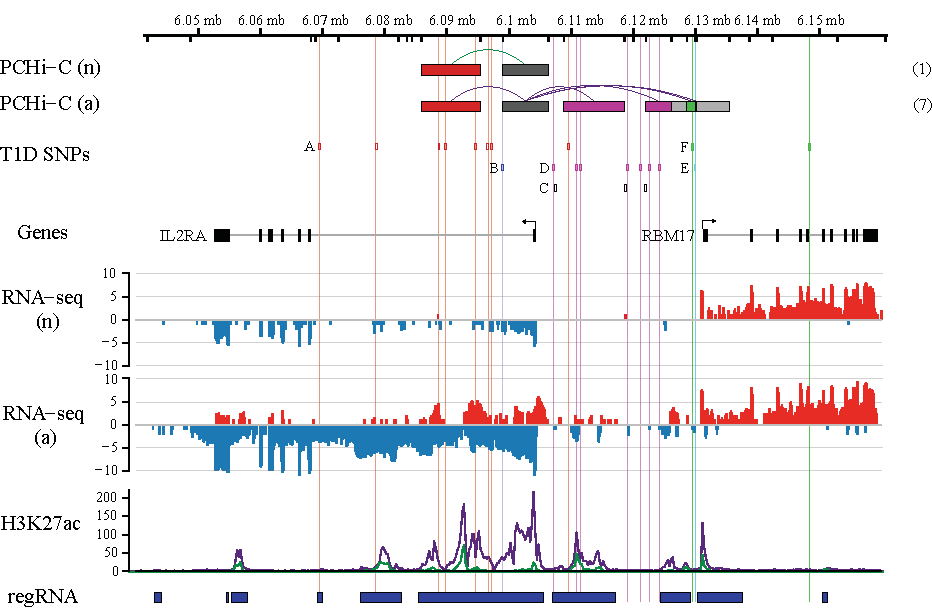
\includegraphics[width=\textwidth]{il2ra_ase_region.pdf}
\caption{PCHi-C interactions link the \textit{IL2RA} promoter to autoimmune disease associated genetic variation which leads to expression differences in \textit{IL2RA} mRNA. (n) and (a) refer to non activated and activated CD4$^+$ T cells respectively. Numbers in parentheses on the right hand side represent number of interactions observed. Labels `A' to `F' indicate sets of SNPs likely to contain a single causal disease variant.  Figure prepared by Tony Cutler, Arcadio Rubio Garcia and Chris Wallace.}
\label{fig:il2ra_ase_reg}
\end{figure}

\begin{figure}[h]
\centering
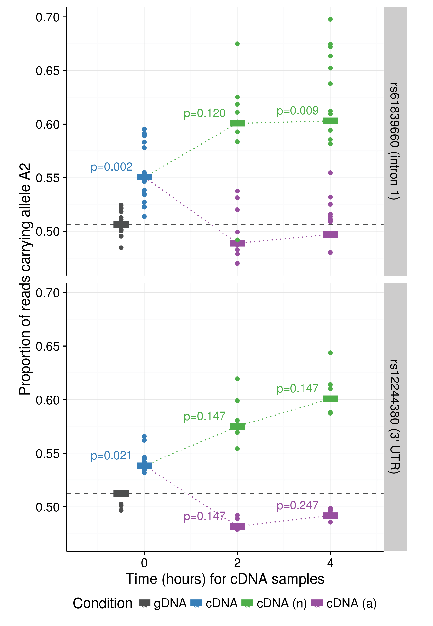
\includegraphics[width=0.6\textwidth]{il2ra_ase_tc.pdf}
\caption{\textit{IL2RA} allele specific expression in CD4$^{+}$ T cells for two putative causal variants identified by fine mapping and PCHi-C integration. Bar colour encodes DNA collected under different conditions. Black indicates genomic DNA, we expect this to be equally shared between alleles. Blue indicates cDNA collected a time zero. Green and purple bars indicate cDNA allele read counts collected under non activated and activated conditions. Figure prepared by Chris Wallace.}
\label{fig:il2ra_ase_tc}
\end{figure}

\section{Limitations}
%write about heterogenous cell populations and the effect that this could have.
There are a number of limitations with the current approaches that I have developed. Firstly the fine mapping approach employed assumes for a given region a simplified model of a single underlying causal variant. I demonstrate that this does have an effect on gene prioritisation but further work is required to how whether the genes prioritised using GUESSFM are in fact better candidates for functional follow up.

Another limitation is the thresholded approach to CHiCAGO scores that are used to call interactions. All of the methods developed so far use a threshold score of 5, so that an interaction with a score of 4.99 will be omitted. Future approaches might investigate methods for incorporating promoter interaction scores in both \textit{blockshifter} and COGS methods. One approach might be to look at techniques that utilise CHiCAGO scores across multiple tissues for a given interaction to adjust local FDR. 

COGS assumes that coding variation affects gene within which it is located, however studies in model organisms~\citep{LawrieMesserHershbergEtAl2013} and in humans~\citep{StergachisHaugenShaferEtAl2013} indicate that coding variation can fulfil a dual role in the regulation of genes. With this in mind, questions include whether such variation has a cis effect on other genes by functioning as regulatory DNA as well as whether we can improve the granularity of coding variant hypothesis by further subdivision (e.g. non-synonymous and synonymous).

One significant problem with these analysis is that resolution is limited by \textit{Hind}III restriction fragment length. This manifests in two main ways, firstly there is a blind spot for observing shorter range interactions that involve \textit{Hind}III fragments and adjoining baited interactions. I have attempted to capture these as `promoter' regions (Figure \ref{fig:cogs}) however integration with functional annotation might provide further resolution and identify functional hypothesis for mechanisms for further study. The second more pernicious issue is that many baited fragments are promiscuous in that they contain promoter regions for more than one gene. If we consider just protein coding genes then of 16,608 baits 3,009 ($18\%$) contain multiple promoters from different genes, if we include all transcriptional start site annotations in Ensembl (Version 75) then this rises to 6,703 ($40\%$). In reality, even this is a conservative estimate due to the incomplete annotation of the non-coding genome. For these promiscuous baits it is impossible to resolve which promoter or promoters are involved in the chromatin looping, using PCHI-C data alone. 

Excluding single cell implementations all genomic technologies give an average of the molecular events across the (somtimes mixed) population of cells being assayed. In the case of immune subsets this is particularly relevant as broad categories, such as CD4$+$ T cells will be heterogeneous containing further subdivisions that may or may not be relevant for disease biology. It is important to bear this in mind when considering PCHi-C maps as without single cell profiling it is impossible to resolve whether interactions are common across the assayed tissue type or are specific to an underlying and as yet unsorted subset.

\chapter{Future Work}

\section{Genomic annotation assisted fine mapping} 
In this report I demonstrate that the integration of high resolution three dimensional chromatin maps with genetic data can inform the biology of autoimmune disease susceptibility. Increasingly high quality genomic datasets on primary human tissues are becoming available. I have shown that both non activated and activated CD4$^{+}$ T cells are of particular interest and  have access to CHiP-Seq and total RNA-Seq for these tissues. Future work will explore whether these annotations can be used as input to intergrative methods such as \textit{fgwas} to increase fine mapping resolution. I will start with autoimmune datasets for which I have access to GWAS summary statistics and use \textit{fgwas} to integrate functional annotations. A concern with \textit{fgwas} is that it relies on extensive cross validation to overcome it's reliance on a single training set, to overcome this I will use the enrichment parameters generated from application to GWAS and use these to compute variable prior probabilities for dense fine mapping information using equations \ref{eqn:fgwas_var_prior} and \ref{eqn:fgwas_var_prior}. These  prior probabilities can be used to compute `annotation aware' posterior probabilities for a variant to be causal. I will use these as input into COGS to understand if and how this alters the genes prioritised. Depending on the outcome of this it might be worth examining RiVIERA~\citep{LiKellis2016} that can make use the covariance across related traits.

% need to state what datasets we might use.

\section{Improving target gene selection}
Understanding how fine scale genetic architecture affects COGS scores is key to their interpretation, for example ascertaining a suitable threshold for gene prioritisation. One approach requires curation of a number of non coding,  causal variants with convincing functional validation for a target gene and tissue context. Unfortunately such examples are rare and so investigation of the effect of parameters such as effect size and minor allele frequency on COGS score is limited. One possible solution is to accurately simulate GWAS based on predifined parameters and causal variants and use this as the input to assess COGS scores at specific intervals or genome wide. Using software developed by Mary Fortune that allows the accurate simulation of GWAS statistics for a given interval I will generate simulated GWAS summary statistics to allow me to understand how various parameters affect the specificity and sensitivity of COGS and any extensions I develop. 



My analysis to date has concentrated on protein coding genes as these have the most mature and complete annotation, however,  recent work has suggested a role for non coding genes in the modulation of autoimmune disease susceptibility ~\citep{Castellanos-RubioFernandez-JimenezKratchmarovEtAl2016}. 

% Need to add more detail as to how Mary's software works and what parameters I intend to look at 

One possible naive solution is to integrate context specific expression data to match genes expressed in that context to possible context specific interactions. This leads on to another possible extension which is to extend prioritisation to include annotated non coding genes as a recent study suggests that these modulate autoimmune disease susceptibility~\citep{Castellanos-RubioFernandez-JimenezKratchmarovEtAl2016}.

\section{Application of COGS scores to the full PCHiC dataset}
Having shown evidence that the COGS tissue specific prioritisation score is useful, I have begun the process of applying it across all traits to all 17 tissue types. For each trait it should be possible to generate a decision tree as in Figure \ref{fig:AHR_dend}. If this is successful I would like to examine metrics for comparing tree structures and therefore inter trait relationships (Figure \ref{fig:RA_dend}).

\begin{figure}[ht]
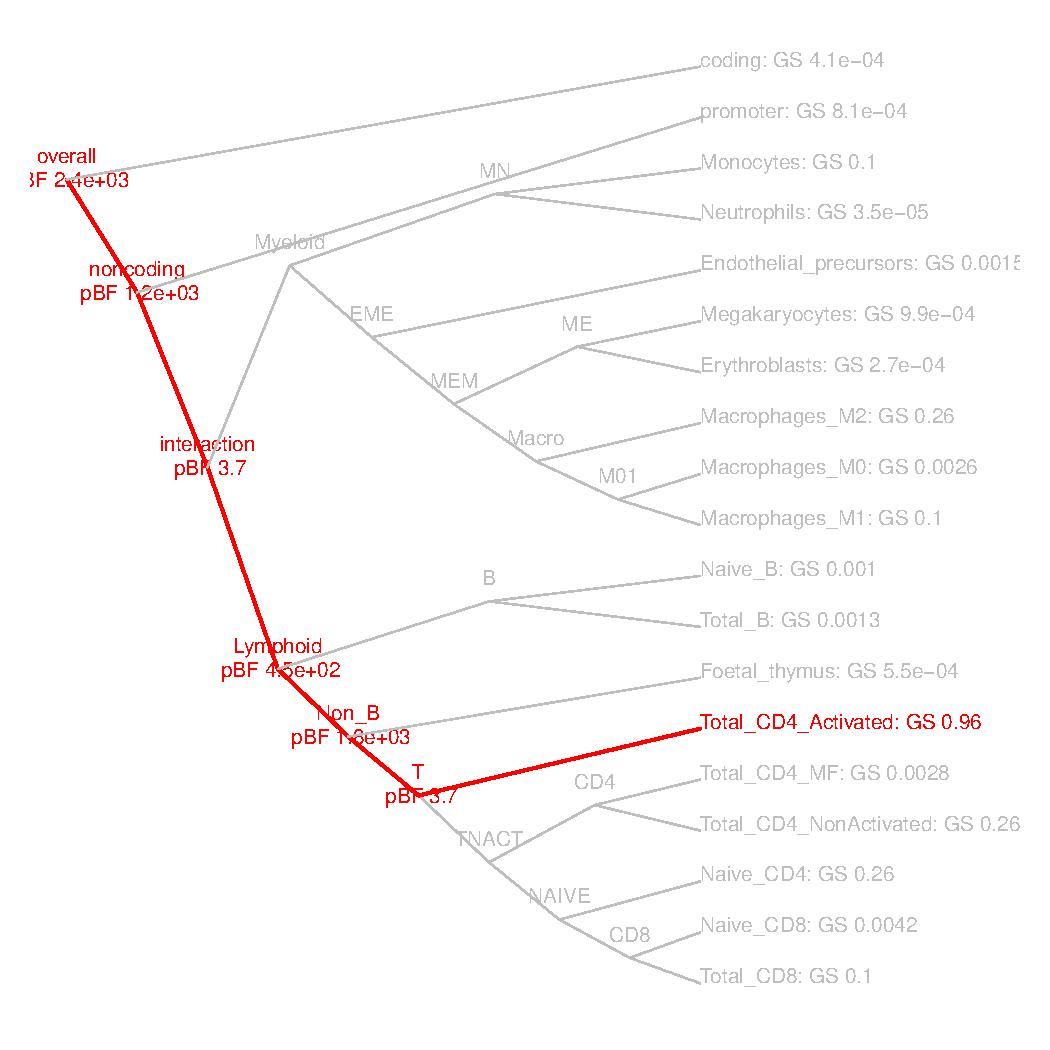
\includegraphics[width=0.7\textwidth]{AHR_dend.pdf}
\caption{COGS decision dendrogram using rheumatoid arthritis data from Okada et al and PCHi-C maps from 17 haematopoietic cell types for the \textit{AHR} gene. The red edges denote the path taken by COGS through the binary decision tree. Each node is labelled with pseudo Bayes factors(pBF). Terminal nodes are labelled with the tissue/annotation specific gene score(GS) }
\label{fig:AHR_dend}
\end{figure}

%\begin{figure}[ht]
%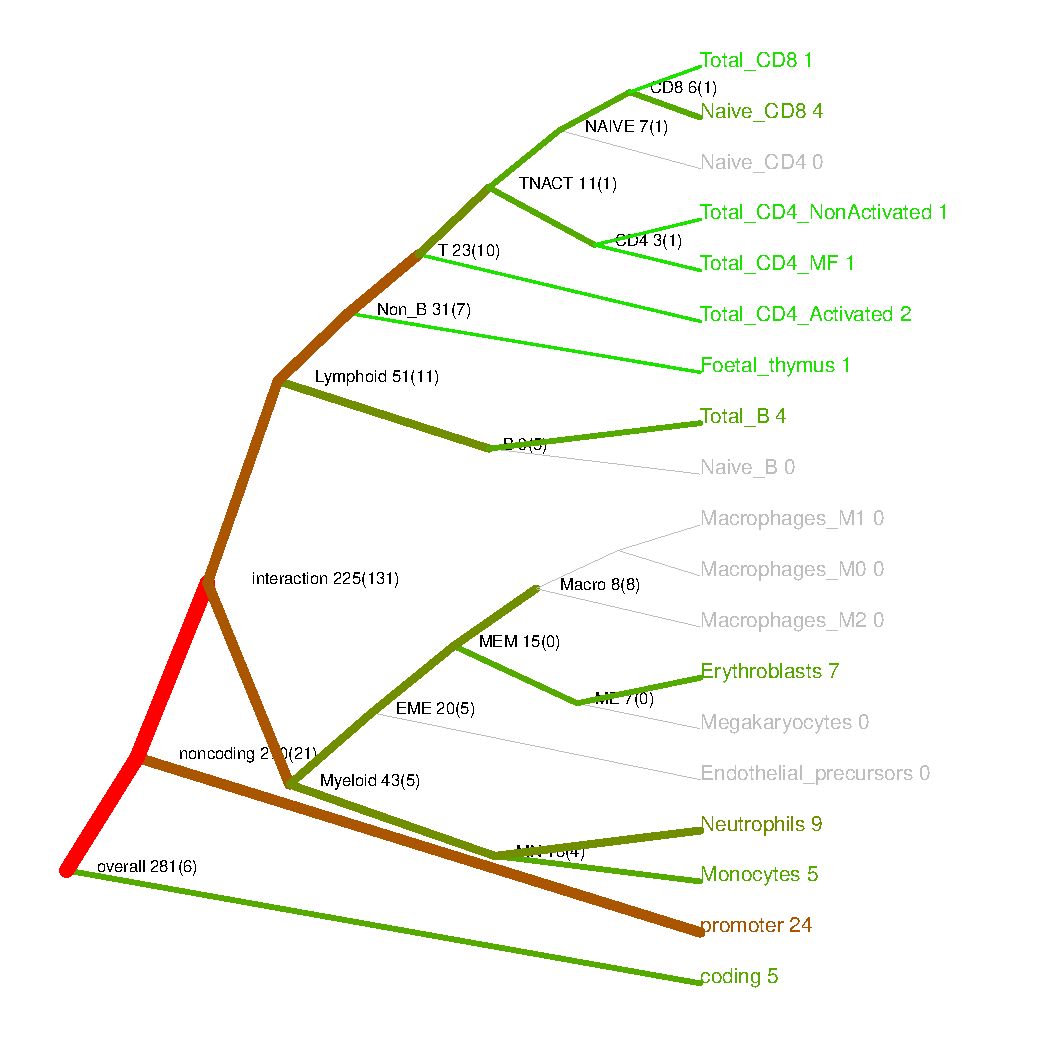
\includegraphics[width=\textwidth]{RA_dend.pdf}
%\caption{COGS decision dendrogram for all prioritised protein coding genes (GS $> 0.5$) using rheumatoid arthritis data from Okada et al and PCHi-C maps from 17 haematopoietic cell types. Edges are coloured based on number of genes flowing between connected nodes. Nodes are marked with the total number of genes at a node and in brackets the number of genes that are assigned to that node.}
%\label{fig:RA_dend}
%\end{figure}

%We should perhaps do this - kind of done - slightly worried about the missing data.
%There are a number of assumptions that are made for these data that require further investigation of their validity. Firstly for traits where only summary GWAS statistics are available we assume a single causal variant for an LD block, one outstanding question is to what effect this has on COGS scores. I aim to do this by comparing traits where we have summary statistics and genotype data and comparing COGS scores of genes between PMI and GUESSFM methods. 

%\section{Comparison with Hi-C defined TAD boundaries}
%So far it is unclear as to how much information is gained in gene prioritisation using promoter capture Hi-C over classical Hi-C. Csilla Varnai and Michiel Thiecke have generated TAD domain boundaries for 8 of the 17 cell types assayed using conventional Hi-C libraries. I will use these to generate pseudo interaction matrices whereby within each TAD the promoter of all genes interacts with every fragment, excepting the baited fragment, and those bounding it for a given gene within a TAD. For these tissues for which Hi-C libraries are available I will also compute gene scores using COGS and analyse the differences to see whether information is gained from using promoter-capture Hi-C over classical Hi-C. 


\section{Integrating other annotations into COGS}

PMI assumes a fixed prior for all SNPs however recent work~\citep{Pickrell2014-xs} using Bayesian hierarchical frameworks demonstrates a method by which we can estimate variable priors for each SNP based on other sources of annotation. In the hierarchical method implemented by \textit{fgwas} for a given SNP the prior probability for association, $\pi_{ik}$, varies depending on the enrichment of annotations, $\lambda_{l}$. 

\begin{equation}
	\pi_{ik} = \frac{e^{x_{i}}}{\sum_{j \in S_k}e^{x_{j}}}
\end{equation}

$x_i$ is the sum of the effect of all the annotations that the $i^{th}$ SNP overlaps as shown below.  Here $\lambda{i}$ is the effect of annotation $l$ and $I_{il}$ is and indicator function as to whether SNP $i$ overlaps annotation $l$.  

\begin{equation}
	x_{i} = \sum_{l=1}^{L_{2}} \lambda_{l}I_{il}
\end{equation}

Initially I would use further information on $CD4^{+}$ T cells including various histone-modification marks and methylation data alongside public ally available annotations to compute $\lambda_{l}$ using \textit{fgwas}.
 Using a model including the most relevant annotations these $x_{i}$ values could also be applied to compute variable priors ($\pi_{i}$) for dense ImmunoChip summary statistics. These more annotation aware posterior probabilities will then be input into COGS to see how this alters gene prioritisation. If this was successful I would look into the incorporation of other BLUEPRINT annotations across all 31 traits.
 
 %what about BLOCKSHIFTER ? If we add variable priors is this good or bad ? I guess in a non efficient way it gives you conditional enrichment ?  

 \section{blockshifter development - perhaps omit}
 
Demonstrating the enrichment of an annotation for associated variants robustly in the presence of correlation is challenging. Correlation, occurring through linkage disequilibrium between SNPs and between genomic annotations,  has the effect of inflating the underlying text statistic and must be carefully adjusted for. The \textit{blockshifter} approach does this using a mixture of circularised and weighted permutation techniques using underlying \textit{Hind}III fragments as atomic units to define underlying block structure. I will investigate the utility of \textit{blockshifter} outside of the PCHiC initially looking at it's performance using (un)activated CD4$^{+}$ T cell ChIP-Seq data sets. In this case I am not limited to \textit{Hind}III but will assay the performance of more frequent cutters (e.g. \textit{SspI}) in terms of results and computational efficiency.
%Can the RF assumptions employed for BS be used as a more general purpose enrichment tool ?
%For COGS can we use fgwas to create variable priors to help increase the resolution ? Also not a big fan of CHiCAGO thresholding approach is there a way we can extend to include interaction probabilities ?

\section{Tissue specific gene set enrichment analysis}
TODO

\section{Data driven discovery of relevant COGS score thresholds}
TODO


\section{Future Directions}
In the longer term I hope to collaborate with clinicians to build promoter capture Hi-C maps of relevant tissues in disease and healthy states. Controlling for variation between individuals in this context is paramount, thus employing strategies to overcome this within the bounds of the economic and technical limitations is important. One strategy is to compare diseased and healthy tissue within the same individual, taken at the same time point to  look for differences in interactions, an example of this might be in juvenile idiopathic arthritis (JIA), here the diseased tissue is known and samples, in the form of synovial fluid drains for are available. PCHi-C results generated from CD4$+$ T cells isolated from the same individual might be compared with those isolated from the periphery. Another complimentary strategy for systemic autoimmune disease where diseased tissue is challenging to collect is to take a longitudinal approach, here patients presenting with a disease are assayed, with further follow up assays collected over time taking into account any therapeutic interventions. Genomic comparison between time points is then conducted to look for differential interactions that might be related to disease prognosis. Further evidence of for a genes involvement in autoimmune disease susceptibility might come from adapting the methods previously described to work with rare variants. For this work one could use gene level variant aggregation tests~\citep{LeeTeslovichBoehnkeEtAl2013} and then use genotype data from primary immune disorders collected as part of the BRIDGE study, PCHiC data would be used to assign variants to genes allowing the integration of both coding and non-coding variation.

\appendix

	%\begin{savenotes}
{\begin{table}[ht]
\caption{Summary of PCHi-C datasets used in this study. Adapted from Javierre et al. (Under review)}
\centering
%\begin{tabularx}{\linewidth}{l l r l l }
%\begin{tabularx}{\linewidth}{X l r l l }
{\tabulinesep=1.2mm
\begin{tabular}{| L{3cm} | C{2cm} | C{2cm} | C{2.6cm} | C{2cm} | }
  \hline
 \rowcolor{white}
 Cell type & Acronym & Biological replicates & Unique captured read pairs & Detected interactions \\
  \hline
 Megakaryocytes & MK &   4 & 653,848,788 & 150,203 \\
 Erythroblasts & Ery &   3 & 588,786,672 & 144,771 \\
 Neutrophils & Neu &   3 & 736,055,569 & 131,609 \\
 Monocytes & Mon &   3 & 572,357,387 & 151,389 \\
 Macrophages M0 & M$\phi0$ &   3 & 668,675,248 & 163,791 \\
 Macrophages M1 & M$\phi1$ &   3 & 497,683,496 & 163,399 \\
 Macrophages M2 & M$\phi2$ &   3 & 523,561,551 & 173,449 \\
 Endothelial Precursors & EndP &   3 & 420,536,621 & 141,382 \\
 Naive B cells & nB &   3 & 629,928,642 & 171,439 \\
 Total B cells & tB &   3 & 702,533,922 & 183,119 \\
 Fetal Thymus & FetT &   3 & 776,491,344 & 145,577 \\
 Naive CD4+ T cells & nCD4 &   4 & 844,697,853 & 192,048 \\
 Total CD4+ T cells & tCD4 &   3 & 836,974,777 & 166,668 \\
 Non-Activated Total CD4+ T cells & naCD4 &   3 & 721,030,702 & 177,371 \\
 Activated Total CD4+ T cells & aCD4 &   3 & 749,720,649 & 188,714 \\
 Naive CD8+ T cells & nCD8 &   3 & 747,834,572 & 187,399 \\
 Total CD8+ T cells & tCD8 &   3 & 628,771,947 & 183,964 \\
 \hline
 \hline
 \rowcolor{gray!50}
 Total & & & 11,299,489,740 & 708,007\tablefootnote{Unique interactions captured in at least one cell type} \\
 \hline
\end{tabular}}
\label{tab:pints}
\end{table}
\addtocounter{footnote}{+1}
}
%\end{savenotes}
	\begin{landscape}
	 	
%\begin{table}[ht]
\begin{center}

\centering
\begin{longtable}{| L{5cm} | C{1.2cm} | C{1cm} | C{1.5cm} | C{1.5cm} | C{1.5cm} | L{2.5cm} | R{1.5cm} | L{4cm} |}
\caption{Summary of GWAS summary statistics used in this study}\label{tab:gwasm}\\
  \hline\rowcolor{white}   Trait & Acronym & Cases & Controls & Study Type & PMID & First Author(Date) & \# SNPs  & Source \\ \hline \hline  
  \endfirsthead
  \hline  \rowcolor{white} Trait & Acronym & Cases & Controls & Study Type & PMID & First Author(Date) & \# SNPs  & Source \\ \hline \hline 
  \endhead
  \hline \rowcolor{white} \multicolumn{9}{|r|}{{Continued on next page}} \\ \hline 
  \endfoot
  \rowcolor{white}\hline \hline 
  \endlastfoot

Platelet volume & PV & 18600 &  & QUANT & 22139419 & Gieger(2011) & 2231438  & N Soranzo personal communication \\
Platelet count & PLT & 48666 &  & QUANT & 22139419 & Gieger(2011) & 2206665  & N Soranzo personal communication \\
Mean corpuscular volume & MCV & 4627 &  & QUANT & 19820697 & Soranzo(2009) & 2156669  & N Soranzo personal communication \\
Packed cell volume & PCV & 4627 &  & QUANT & 19820697 & Soranzo(2009) & 2009357  & N Soranzo personal communication \\
Red blood cell count & RBC & 4627 &  & QUANT & 19820697 & Soranzo(2009) & 2091590  & N Soranzo personal communication \\
Haemoglobin & HB & 4627 &  & QUANT & 19820697 & Soranzo(2009) & 1640923  & N Soranzo personal communication \\
Mean corpuscular haemoglobin & MCH & 4627 &  & QUANT & 19820697 & Soranzo(2009) & 1904974  & N Soranzo personal communication \\
Mean corpuscular haemoglobin concentration & MCHC & 4627 &  & QUANT & 19820697 & Soranzo(2009) & 2070334  & N Soranzo personal communication \\
Ulcerative colitis Anderson & UC & 6687 & 19718 & CC & 21297633 & Anderson(2011) & 1399283  & \url{http://www.immunobase.org} \\
Multiple sclerosis IMSGC & MS & 9772 & 17376 & CC & 21833088 & IMSGC(2011) & 463628  & \url{http://www.immunobase.org} \\
Type 1 diabetes Barrett & T1D & 8000 & 8000 & CC & 19430480 & Barrett(2009) & 789849  & \url{http://www.immunobase.org} \\
Celiac disease DuBois & CEL & 4533 & 10750 & CC & 20190752 & Dubois(2010) & 509768  & \url{http://www.immunobase.org} \\
Crohn's disease immunobase & CD & 6333 & 15056 & CC & 21102463 & Franke(2010) & 950208  & \url{http://www.immunobase.org} \\
Rheumatoid arthritis Okada & RA & 14361 & 43923 & CC & 24390342 & Okada(2014) & 8513749  & \url{http://plaza.umin.ac.jp/\~okada/datasource/files/GWASMetaResults/RA\_GWASmeta\_European\_v2.txt.gz} \\
Type 2 diabetes & T2D & 12171 & 56860 & CC & 22885922 & Morris(2012) & 2075585  & \url{http://diagram-consortium.org/downloads.html} \\
Height & HT & 253288 &  & QUANT & 25282103 & Wood(2014) & 1927160  & \url{https://www.broadinstitute.org/collaboration/giant/images/0/01/GIANT\_HEIGHT\_Wood\_et\_al\_2014\_publicrelease\_HapMapCeuFreq.txt.gz} \\
Tryglycerides & TG & 96598 &  & QUANT & 20686565 & Teslovich(2010) & 2304026  & \url{http://csg.sph.umich.edu/abecasis/public/lipids2010/TG2010.zip} \\
High density lipoprotein & HDL & 99900 &  & QUANT & 20686565 & Teslovich(2010) & 2322449  & \url{http://csg.sph.umich.edu/abecasis/public/lipids2010/HDL2010.zip} \\
Low density lipoprotein & LDL & 95454 &  & QUANT & 20686565 & Teslovich(2010) & 2298548  & \url{http://csg.sph.umich.edu/abecasis/public/lipids2010/LDL2010.zip} \\
Total Cholesterol & TC & 100184 &  & QUANT & 20686565 & Teslovich(2010) & 2323152  & \url{http://csg.sph.umich.edu/abecasis/public/lipids2010/TC2010.zip} \\
Glucose sensitivity BMI adjusted & GLC\_B & 58074 &  & QUANT & 22581228 & Manning(2012) & 2622994  & \url{ftp://ftp.sanger.ac.uk/pub/magic/MAGIC\_Manning\_et\_al\_FastingGlucose\_MainEffect.txt.gz} \\
Glucose sensitivity & GLC & 58074 &  & QUANT & 22581228 & Manning(2012) & 2622996  & \url{ftp://ftp.sanger.ac.uk/pub/magic/MAGIC\_Manning\_et\_al\_FastingGlucose\_MainEffect.txt.gz} \\
Insulin sensitivity BMI adjusted & INS\_B & 51750 &  & QUANT & 22581228 & Manning(2012) & 2621974  & \url{ftp://ftp.sanger.ac.uk/pub/magic/MAGIC\_Manning\_et\_al\_lnFastingInsulin\_MainEffect.txt.gz} \\
Insulin sensitivity & INS & 51750 &  & QUANT & 22581228 & Manning(2012) & 2621977  & \url{ftp://ftp.sanger.ac.uk/pub/magic/MAGIC\_Manning\_et\_al\_lnFastingInsulin\_MainEffect.txt.gz} \\
Femoral neck bone mineral density & FNBMD & 32961 &  & QUANT & 22504420 & Estrada(2012) & 2473840  & \url{http://www.gefos.org/sites/default/files/GEFOS2\_FNBMD\_POOLED\_GC.txt.gz} \\
Lumbar spine bone mineral density & LSBMD & 32961 &  & QUANT & 22504420 & Estrada(2012) & 2463611  & \url{http://www.gefos.org/sites/default/files/GEFOS2\_LSBMD\_POOLED\_GC.txt.gz} \\
Diastolic blood pressure & BP\_D & 69395 &  & QUANT & 21909115 & ICBP(2011) & 2460847  & \url{http://www.georgehretlab.org/ICBP-summary-Nature.csv.gz} \\
Systolic blood pressure & BP\_S & 69395 &  & QUANT & 21909115 & ICBP(2011) & 2460847  & \url{http://www.georgehretlab.org/ICBP-summary-Nature.csv.gz} \\
Body Mass Index & BMI & 322200 &  & QUANT & 25673413 & Locke(2015) & 1984096  & \url{https://www.broadinstitute.org/collaboration/giant/images/1/15/SNP\_gwas\_mc\_merge\_nogc.tbl.uniq.gz} \\
Systemic Lupus Erythrematosis & SLE & 4036 & 6959 & CC & 26502338 & Bentham(2015) & 7734064  & \url{http://www.immunobase.org} \\
Primary Billiary Cirrhosis & PBC & 2764 & 10475 & CC & 26394269 & Cordell(2015) & 1134133  & \url{http://www.immunobase.org} \\
  
\end{longtable}
\end{center}
%\end{table}
	\end{landscape}
	
%\begin{table}[ht]
\begin{center}

\centering
\begin{longtable}{| L{5cm} | R{1.2cm} | R{1cm} | L{1.5cm} |}
\caption{Summary of differentially expressed genes from~\citet{PetersLyonsLeeEtAl2016} with COGS gene scores $>$ 0.5 for ulcerative colitis (UC) and Crohn's Disease (CD)}
\label{tab:ibd_genes}\\
  \hline\rowcolor{white}   Gene Name & COGS score & DE P$_{adj}$ & Disease \\ \hline \hline  
  \endfirsthead
   \hline\rowcolor{white}   Gene Name & COGS score & DE P$_{adj}$ & Disease \\ \hline \hline  
  \endhead
  \hline \rowcolor{white} \multicolumn{4}{|r|}{{Continued on next page}} \\ \hline 
  \endfoot
  \rowcolor{white}\hline \hline 
  \endlastfoot

FAIM3 & 1.000 & 0.000 & UC \\ 
COX4I1 & 1.000 & 0.036 & UC \\ 
RPS24 & 1.000 & 0.011 & CD \\ 
IKZF1 & 0.999 & 0.001 & CD \\                              
ACSS1 & 0.999 & 0.017 & UC \\ 
CHD1 & 0.988 & 0.032 & CD \\ 
CD274 & 0.987 & 0.002 & CD \\ 
ROPN1L & 0.944 & 0.042 & UC \\ 
ADO & 0.941 & 0.006 & CD \\ 
 TFAM & 0.939 & 0.001 & CD \\ 
 ETS1 & 0.934 & 0.001 & UC \\ 
 MIDN & 0.927 & 0.011 & CD \\ 
 SBNO2 & 0.926 & 0.000 & CD \\ 
 IPMK & 0.922 & 0.028 & CD \\ 
 RQCD1 & 0.914 & 0.038 & UC \\ 
 STK32B & 0.894 & 0.022 & UC \\ 
 CTDSP1 & 0.877 & 0.008 & UC \\ 
 ADAM10 & 0.854 & 0.006 & UC \\ 
 MYC & 0.836 & 0.034 & CD \\ 
 FCGR2A & 0.836 & 0.021 & UC \\ 
 FCRLA & 0.835 & 0.018 & UC \\ 
 SGMS1 & 0.835 & 0.000 & UC \\ 
 CD244 & 0.823 & 0.003 & CD \\ 
 PIM3 & 0.822 & 0.001 & UC \\ 
 BCL6 & 0.811 & 0.001 & UC \\ 
 RTP2 & 0.800 & 0.043 & UC \\ 
 RASGRP1 & 0.795 & 0.005 & CD \\ 
 IKZF3 & 0.793 & 0.000 & UC \\ 
 LYRM7 & 0.771 & 0.001 & UC \\ 
 DGKD & 0.758 & 0.004 & CD \\ 
 CHRNE & 0.737 & 0.041 & UC \\ 
 ARRB2 & 0.717 & 0.001 & UC \\ 
 PIP4K2C & 0.686 & 0.009 & UC \\ 
 ADAM9 & 0.684 & 0.000 & UC \\ 
 GATA3 & 0.679 & 0.031 & UC \\ 
 PAPD7 & 0.659 & 0.007 & UC \\ 
 MFF & 0.658 & 0.020 & UC \\ 
 IGF2 & 0.649 & 0.049 & UC \\ 
 STK36 & 0.634 & 0.013 & UC \\ 
 GPX4 & 0.631 & 0.000 & CD \\ 
 BEST1 & 0.627 & 0.001 & CD \\ 
 ATG4D & 0.626 & 0.017 & CD \\ 
 AGAP2 & 0.621 & 0.017 & UC \\ 
 SMAD3 & 0.612 & 0.013 & CD \\ 
 MRPL4 & 0.599 & 0.017 & CD \\ 
 MARCH9 & 0.594 & 0.003 & UC \\ 
 MAN2A2 & 0.591 & 0.038 & CD \\ 
 GALC & 0.589 & 0.001 & CD \\ 
 CDK4 & 0.588 & 0.014 & UC \\ 
 MLC1 & 0.575 & 0.031 & CD \\ 
 DSE & 0.573 & 0.000 & UC \\ 
 BCL2 & 0.565 & 0.015 & UC \\ 
 FBL & 0.561 & 0.001 & UC \\ 
 C9orf37 & 0.543 & 0.001 & UC \\ 
 DPP7 & 0.542 & 0.047 & UC \\ 
 SSNA1 & 0.542 & 0.000 & UC \\ 
 PHPT1 & 0.542 & 0.007 & UC \\ 
 CCDC183 & 0.542 & 0.012 & UC \\ 
 ABCA2 & 0.542 & 0.021 & UC \\ 
 SCAMP3 & 0.529 & 0.020 & CD \\ 
 TTC1 & 0.523 & 0.045 & UC \\ 
 ZBTB49 & 0.520 & 0.047 & UC \\ 
 CD55 & 0.517 & 0.002 & UC \\ 
 FYB & 0.508 & 0.008 & CD \\ 
 ATF6 & 0.504 & 0.003 & UC \\ 
   \hline
\end{longtable}
\end{center}
%\end{table}
\bibliographystyle{genomeresearch}
%\bibliographystyle{plain}
\bibliography{first_year_report}

\end{document}
